\chapter[Modelado Procedimental de Geometrías Porosas]{Modelado Procedimental de Geometrías de Miga de Pan y Otros Materiales Porosos}

\section{Introducción y Motivación} % (Películas de Animación)
Como fue explicado en la motivación de esta tesis, determinados materiales recibieron menor atención en la literatura científica, debido entre otros factores, a las dificultades presentes	 en el modelado, a los excesivos costos computacionales, y/o a la necesidad de utilización del material en aplicaciones prácticas.
Con el paso de los a\~nos, la industria del cine y de los video juegos diseñó y aplicó procedimientos artísticos con el fin de subsanar estas deficiencias.
De esta forma, se busc\'o la mayor similitud posible en la apariencia, entre el material sintetizado y el real, sin considerar si el proceso provenía de una simulación física o era el resultado de un procedimiento artístico.

Entre los innumerables ejemplos que se pueden citar, uno particularmente relacionado al trabajo de esta tesis lo constituye la película Ratatouille \cite{Cho2007}.
La misma se desarrolla en un ambiente de cocina, y por lo tanto existen alimentos y materiales naturales que deben ser modelados para ser renderizados.
Debido a la inexistencia de modelos estándar de determinados materiales en la literatura de computación gráfica (comestibles), los artistas y programadores encargados de llevar a cabo la producción visual de la película debieron crear técnicas {\em ad-hoc} para lograr un renderizado realista de los diferentes materiales.
Sin embargo, el éxito visual obtenido no se vio acompañado de una liberación del código que producía dichas imágenes, por lo cual la técnica permaneció para uso privado de la compañía productora, resultando en una difícil reproducción de dichos materiales por parte de terceros.

En este capítulo se busca introducir soluciones a estas problemáticas: por un lado, la falta de modelos fenomenológicos documentados y por lo tanto reproducibles, sobre geometría de migas de panes y otros materiales porosos, y por otro, la utilización de modelos físicos basados en los procesos reales de formación de dichos materiales, los cuales provocan que el resultado sintético posea una mayor similitud visual y estructural a los materiales que se pretenden representar.

En este capítulo presentamos modelos procedimentales que permiten realizar simulaciones de la geometría de la miga de pan.
Como sub-producto presentamos un algoritmo que produce imágenes de texturas bidimensionales de materiales estocásticos como granito y mármol, y otros más estructurados como la madera.

\subsection{Consideraciones sobre el modelado de geometrías porosas}
Como fue discutido en el capítulo anterior, la inmensa variedad de materiales, y sus complejas interacciones con la energía radiante que incide sobre los mismos, han sido un tópico central de investigación en las últimas décadas en Computación Gráfica.
El modelado de la naturaleza en física ha demostrado capturar de manera muy precisa fenómenos de transporte de la luz.
Las aproximaciones computacionales a estos modelos son una de las ramas más investigadas en el renderizado de materiales.
El modelado geométrico de materiales sigue una estrategia de investigación similar. Primero se construye un modelo físico del material, el cual luego se aproxima computacionalmente.
La elección del modelo geométrico depende de cada material, y de la escala de representación buscada.
Esta elección influencia fuertemente el algoritmo de renderizado. 

%Existen dos tipos principales de modelos para capturar la apariencia de materiales: superficies y volúmenes.
%Para esto existen dos ecuaciones principales.
%Por un lado, la ecuación del rendering \cite{Kajiya1986} captura la microgeometría de los materiales y su interacción con la luz en superficies.
%Por otro, la ecuación del rendering de volúmenes \cite{Kajiya1984} modela fenómenos volúmetricos como la transmitancia, la extinción, etc., debido a propiedades del medio (o material).

Si el material a representar presenta características homogéneas (metales, plásticos, y similares), típicamente se lo modela por medio de una superficie \cite{Neumann1999}.
Esta estrategia modela la superficie del material asumiendo distribuciones estadísticas en su microgeometría.
Para lograr capturar detalles mesoscópicos, por ejemplo en el caso de maderas o ladrillos \cite{Lefebvre2000}, una técnica usual consiste en precomputar dichas características en texturas, las cuales luego son mapeadas en la superficie.
La utilización de superficies constituye un enfoque menos costoso computacionalmente, pero por otro lado impone limitaciones al realismo que se puede alcanzar, sobre todo en aquellos detalles que son propios de la estructura a nivel mesoscópico y la interacción de la misma con la luz (por ejemplo luz que pasa a través de agujeros en una superficie).

Siguiendo este razonamiento, la miga del pan constituye un material extremadamente complejo de capturar, modelar y renderizar, debido a la geometría a distintos niveles (microscópico y mesoscópico) y su resultante interacción con la energía radiante.
De esta forma, la utilización de superficies no resulta adecuada, ya que la textura del pan debe su apariencia en gran medida a los fenómenos previamente explicados.
Si bien existen métodos en la literatura que utilizan superficies para representar características mesoscópicas de los materiales como BTFs, las mismas no manejan adecuadamente la interacción lumínica antes mencionada.
Existe un intento en la literatura por suprimir esta falta \cite{Tong2005}.
El método produce imágenes realistas, pero existen muchas dificultades prácticas en la captura, el cómputo y el renderizado.
Estas limitaciones provocan que la utilización de dicho método no sea práctica por el momento.
Además, el método resulta inflexible dado que para cada imagen del material se requiere repetir todo el proceso (dos imágenes distintas del material requieren dos capturas).
Tampoco se pueden obtener cortes del mismo, dada la naturaleza de superficie del método.

Por otro lado, existen numerosas publicaciones que tratan el modelado de materiales mejor adaptados a una representación volumétrica (por ejemplo humo o nubes) \cite{Chentanez2011,Zhou2008}.
La utilización de volúmenes resulta costosa computacionalmente pero presenta varias ventajas.
Una de ellas radica en su independencia de mallas de triángulos, a diferencia de las superficies, evitando las desventajas mencionadas para las mismas.

Finalmente, existe un compromiso al momento de modelar materiales complejos y elegir una representación plausible.
Donde se requiere simplicidad y velocidad (posiblemente tiempo real), se utilizan generalmente superficies, en cambio, si el foto-realismo constituye el objetivo final, resulta más adecuado optar por una representación volumétrica.
En los últimos años esta elección se ve enriquecida por la aparición de hardware paralelo de alta velocidad (placas gráficas o GPUs), ya que un diseño adecuado podría producir imágenes foto-realistas utilizando volúmenes en tiempos interactivos.

En este capítulo proponemos una representación volumétrica para la geometría de la miga de pan.
Existe una metodología volumétrica que simula geometrías estocásticas \cite{Perlin1989}, utilizando funciones algebraicas para construir la geometría.
Sin embargo, la utilización de funciones algebraicas resulta impráctica en el caso de materiales porosos estocásticos, como el pan.

\section[Síntesis de Texturas de Materiales]{Un Framework para la Síntesis de Texturas de Materiales}

La textura característica de la miga de pan emerge como resultado de numerosos procesos.
El crecimiento de la levadura en la masa cruda del pan produce una de las principales transformaciones texturales.
A este proceso le atañe la mayor responsabilidad en la formación de la geometría porosa macroscópica del material.
La observación detallada de binarizaciones de fotografías de cortes en la masa cruda, durante distintas etapas del proceso de leudado y cocción del pan \cite{Scanlon2001}, permite sentar las bases de un algoritmo fenomenológico que responde a este comportamiento.
En dichas imágenes se observa un crecimiento pseudo-aleatorio de burbujas atrapadas en la masa.
La textura final debe su apariencia a un aglomerado de burbujas interconectadas con distintos tamaños y formas.

La implementación de este método constituye el principal motivo de esta sección.
Si bien el objetivo del mismo radica en la producción de geometrías, como sub-producto surgen imágenes o geometrías que recuerdan apariencias típicas de otros materiales.
Al asignárseles colores, permiten obtener imágenes aceptables de los mismos.

Presentamos entonces un método procedimental de generación de texturas de materiales en dos dimensiones, basado en el crecimiento de partículas \cite{Reeves1983}.
Se define una textura como una imagen. o arreglo bidimensional de múltiples usos que almacena información sobre un fenómeno determinado.
En este caso, una textura representará el material directamente, a nivel macroscópico (es decir una imagen del mismo).
La simulación de imágenes de materiales usualmente se presenta en publicaciones separadas en la literatura, dado que los procedimientos que producen distintos materiales se basan en metodologías dispares.
El algoritmo introducido será luego descripto en casos especiales, en la obtención de geometrías de la miga de pan y otros materiales porosos.

\subsection{Sistemas de Partículas}
Un sistema de partículas está compuesto por abstracciones denominadas {\em partículas}, las cuales coexisten en un mismo ambiente.
En un sistema de part\'iculas, las part\'iculas nacen, se desarrollan y mueren, respetando reglas que les son impuestas por el sistema. Estos sistemas intentan modelar la din\'amica del fen\'omeno a trav\'es del tiempo, siendo uno de sus principales intereses mostrar una animaci\'on del mismo \cite{Gao2010, Bagar2010, Lentine2010}.

Se propone utilizar estos sistemas como generadores procedimentales de texturas. Un enfoque similar puede observarse en \cite{Kranidotis98}, aunque el mismo no fue desarrollado en profundidad.
Aquí se sigue una linea de investigaci\'on semejante, presentando un sistema de part\'iculas que est\'a caracterizado por el crecimiento de las mismas en cada iteraci\'on, las cuales ocupan texels (elemento individual de una textura bidimensional, correspondiente a una posición $(u,v)$ dentro de la misma) asign\'andoles colores, pudi\'endose detener al mismo en una iteración arbitraria, obteni\'endose una textura.
Debido a la utilización de una selección aleatoria de los texels vecinos, donde crece cada partícula, las im\'agenes resultantes presentan apariencia estocástica, de manera análoga a materiales naturales.
A trav\'es de la direcci\'on de crecimiento de las part\'iculas se producen distintos patrones visuales.

Es posible representar materiales cl\'asicos como madera, granito y m\'armol, pero tambi\'en otros como mosaicos, pinturas, vegetaci\'on, entre muchos otros.
Un ejemplo de generación procedimental de texturas puede observarse en \cite{Baravalle2010}.
La diferencia principal con el enfoque presentado en este trabajo radica en el mecanismo de generaci\'on, dado que con esta nueva propuesta un {\em proceso temporal} produce los resultados, pudiendo representarse todo el proceso de formaci\'on de un material.
Adem\'as, cada ejecución del algoritmo produce una textura diferente, utilizando los mismos par\'ametros, debido a la naturaleza aleatoria de la generaci\'on (aunque el uso de semillas permite repetir texturas en el caso de requerirse, por ejemplo para generar baldosas id\'enticas).

Se utiliza como plataforma de implementaci\'on a WebGL\footnote{\em http://www.khronos.org/webgl/}, recientemente propuesta por el Khronos Group (Open Standars for Media Authoring and Acceleration), dado que la misma otorga portabilidad al modelo (es posible ejecutarlo en una gran variedad de navegadores independientemente de la plataforma en la que se encuentre la computadora). 
La implementación desarrollada permite incluirlo en aplicaciones gr\'aficas.
Dada la intuitividad de los parámetros del mismo (direcciones de crecimiento, cantidad de partículas iniciales, etc.), los artistas pueden interactuar con el programa, buscando obtener imágenes de distintos materiales.

\subsubsection{Desarrollo}
Inicialmente el sistema consta de un conjunto de part\'iculas $P$
\begin{equation}
P = \{p_{1}, ... , p_{n}\}, n  \in \mathbb{N},
\end{equation}
uno o varios colores {\em RGB}, los cuales pueden tomar las part\'iculas.
\begin{equation}
cols = \{col_{1}, ... , col_{m} \}, m \in \mathbb{N},
\end{equation}
un conjunto de direcciones de crecimiento $D$,
\begin{equation}
D = \{d_{1}, ... , d_{k} \}, k \in \mathbb{N},
\end{equation}
y una grilla $B_{N\times N}, N \in \mathbb{N} $ de texels con colores RGB asociados (inicialmente $(R,G,B)=(0,0,0)$).

Cada elemento del conjunto $P$ posee las siguientes propiedades:
\begin{equation}
p_{i} = \{T_{i}, C_{i}, d_{i}, color_{i}\}, 1 \le i \le n,
\end{equation}
donde:

$T_{i} = \{t_{1}, ... , t_{n_{i}}\}$: conjunto de texels {\em ocupados} por la part\'icula en $B$,

$C_{i} = \{c_{1}, ... , c_{m_{i}}\}$: conjunto de texels {\em contorno} de la part\'icula en $B$,

$d_{i} \in D$: direcci\'on de crecimiento,

$color_{i}$: color {\em RGB} de la part\'icula, con ecuaci\'on \cite{Reeves1983}
\begin{equation}
color_{i} = col_{h} + rand * varcolor,
\label{eqColor}
\end{equation}

\noindent
y donde {\it rand} constituye un n\'umero pseudo-aleatorio uniformemente distribuido entre $-1$ y $1$, $varcolor$ un parámetro en los reales y $col_{h} \in cols$.
Cada $t \in T_{i}$ tiene asociado un color que var\'ia con respecto a $color_{i}$, de similar manera a la ecuaci\'on (\ref{eqColor}).

El {\em contorno} de una part\'icula determina los texels que la misma puede incorporar. 
En cada iteraci\'on, se elige aleatoriamente un texel en $C_{i}$, se lo quita del mismo y se lo incorpora a $T_{i}$.
Luego se actualiza el contorno de acuerdo a $d_{i}$ y al nuevo texel incorporado.
Se repite el proceso $\forall p_{i} \in P$, respetando las siguientes restricciones:
\begin{eqnarray}
\forall p_{i}, p_{j} \in P, t \in T_{i} \Rightarrow t \notin T_{j}, \\
\forall p_{i} \in P, t \in T_{i} \Rightarrow t \notin C_{i}.
\end{eqnarray}

Es decir, si una part\'icula posee un texel en $T_{i}$, ninguna otra lo posee (las part\'iculas son disjuntas), y si una part\'icula posee un texel en $T_{i}$, \'este no est\'a en su contorno.
Las part\'iculas pueden {\em nacer} y {\em morir}, lo cual representa su inclusi\'on o eliminaci\'on de $P$.
Al morir, la part\'icula deja asociados los colores de su conjunto $T_{i}$ en $B$, pudiendo utilizarse posteriormente esta informaci\'on.

%Podemos intentar aplicar estas técnicas al modelado procedimental de texturas. 
En la Fig. \ref{resultados} se observan algunas im\'agenes sintetizadas con esta metodología.
En la primera fila, la primera y cuarta textura muestran patrones con direcci\'on vertical, direcci\'on elegida para evolucionar las part\'iculas.
La \'ultima figura de la segunda fila, muestra part\'iculas que crecen en 3 direcciones posibles: aleatorio ($50\%$), vertical ($25\%$) y horizontal ($25\%$), lo cual demuestra que se posee un control preciso sobre las formas resultantes en las texturas.

En la Fig. \ref{sintesis} se observa un ejemplo de s\'intesis.
De izquierda a derecha, se observan texturas obtenidas en las iteraciones $10$, $150$, $250$, $500$ y $1000$.
En la Fig. \ref{teteras} se observan texturas sintetizadas aplicadas a un objeto mediante mapeo de texturas, mostrando una calidad aceptable para ser utilizadas en aplicaciones gr\'aficas.

La Fig. \ref{muerte} muestra el efecto de muerte de part\'iculas.
Las mismas liberan el espacio en $T_{i}$ dejando asociado su color en $B$, permitiendo que las dem\'as puedan crecer en dichos texels.
De esta forma, puede utilizarse posteriormente la informaci\'on que la misma dej\'o asociada.
En este caso los colores de la part\'icula que libera el espacio y la ocupante fueron mezclados, obteni\'endose im\'agenes que parecen haber sido ``pintadas'' por capas.
%En la Figura \ref{software} se observa el modelo corriendo en un navegador web.


\begin{figure}[t!]
\centering
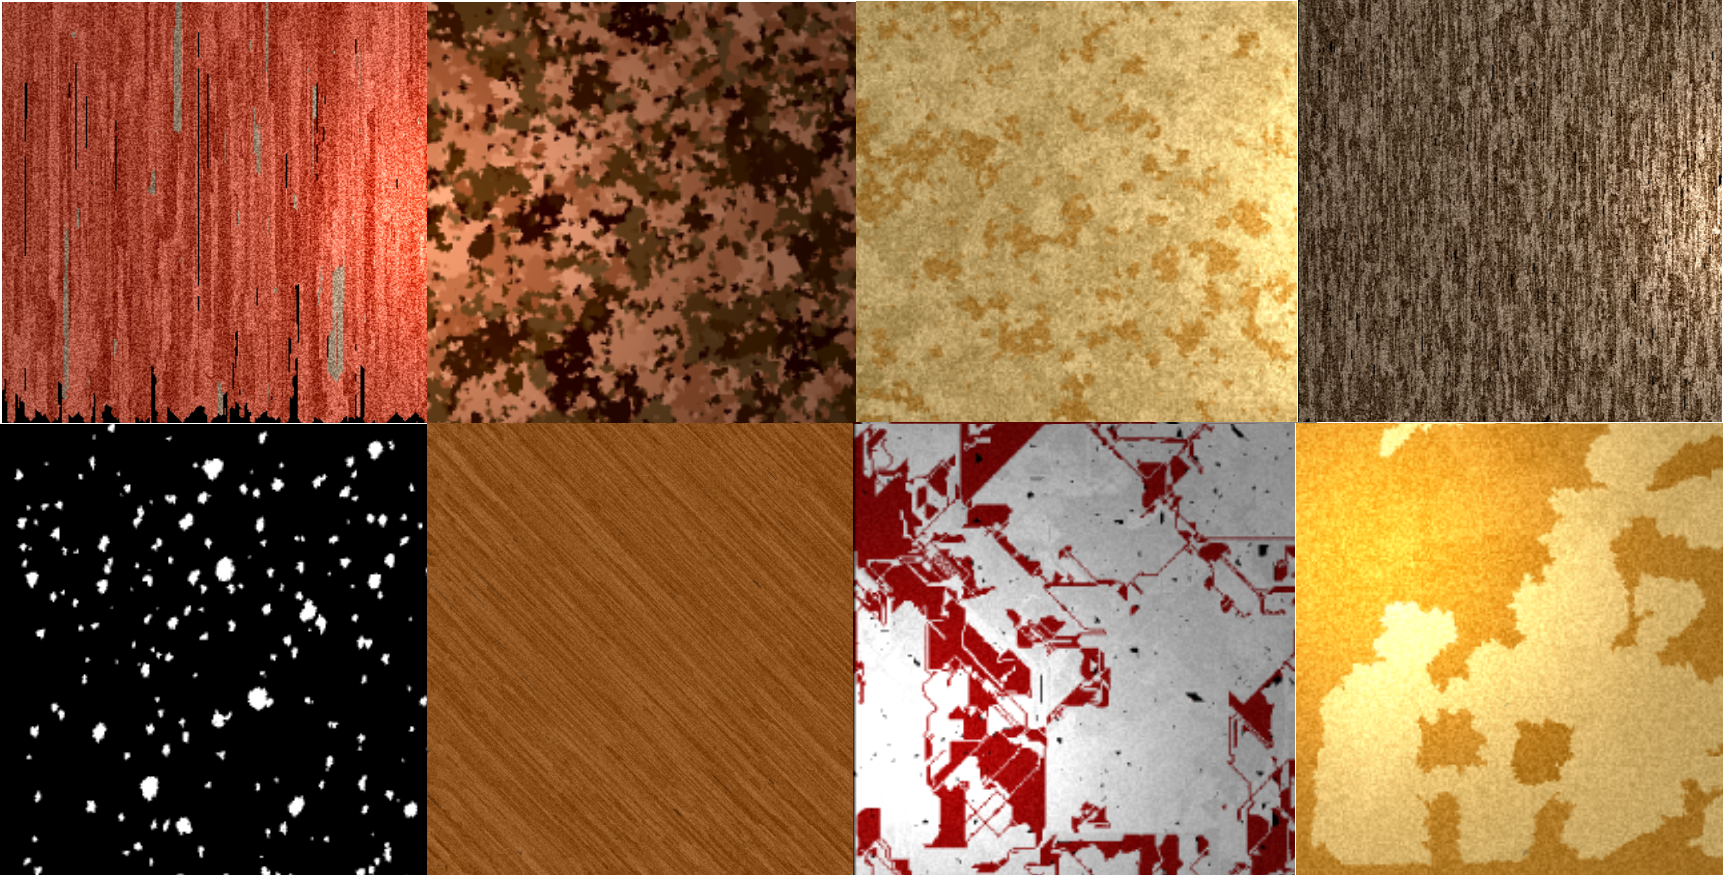
\includegraphics[scale=0.18]{figures/resultados}
\caption{Distintas texturas sintetizadas utilizando sistemas de partículas.}
\label{resultados}
\end{figure}

Se muestra un ejemplo de s\'intesis de una textura en la Fig.~\ref{sintesis}. Deben seleccionarse los siguientes par\'ametros:

\begin{itemize}
\item Par\'ametro {\em cantidad de part\'iculas iniciales}, con valor $100$.
\item Par\'ametro {\em nuevas particulas por iteraci\'on}, con valor $1$.
\item Par\'ametros {\em color 1 y 2 (RGB)}. con colores de ejemplo, uno con la componente verde mayor y otro con mayor componente azul.
\item Par\'ametros {\em direcciones}: aleatorio: $50\%$, diagonal $50\%$.
\item Par\'ametro {\em variaci\'on de color}, con valor 0.1, en una escala [0,1] (ver $varcolor$ en la secci\'on anterior).
\item Par\'ametro {\em variaci\'on de color por part\'icula}, con valor 0.1, en una escala $[0,1]$, el cual determina la variaci\'on del color por texel dentro de la part\'icula.
\end{itemize}

\begin{figure}[t!]
\centering
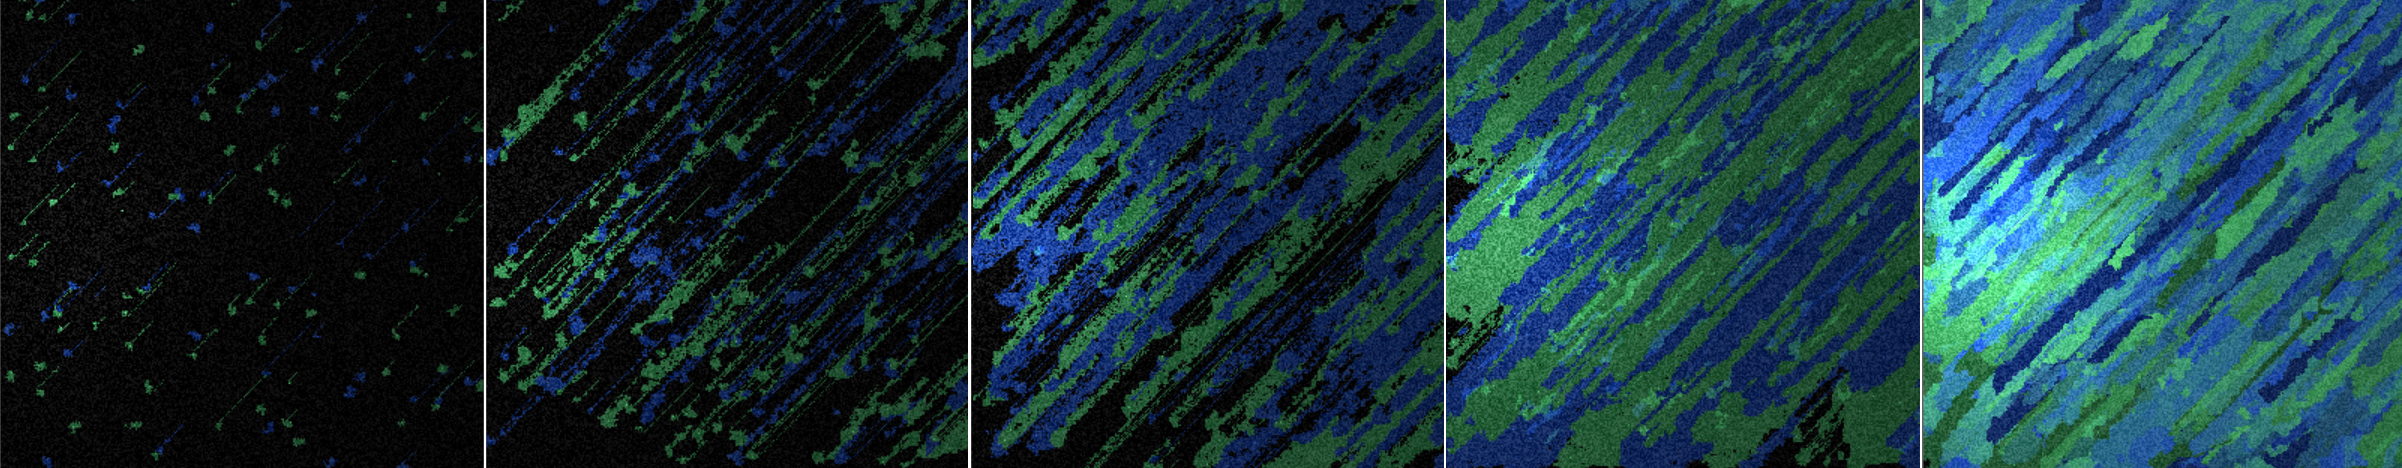
\includegraphics[scale=0.12]{figures/sintesis}
\caption{Ejemplo de s\'intesis de una textura.}
\label{sintesis}
\end{figure}

\begin{figure}[t!]
\centering
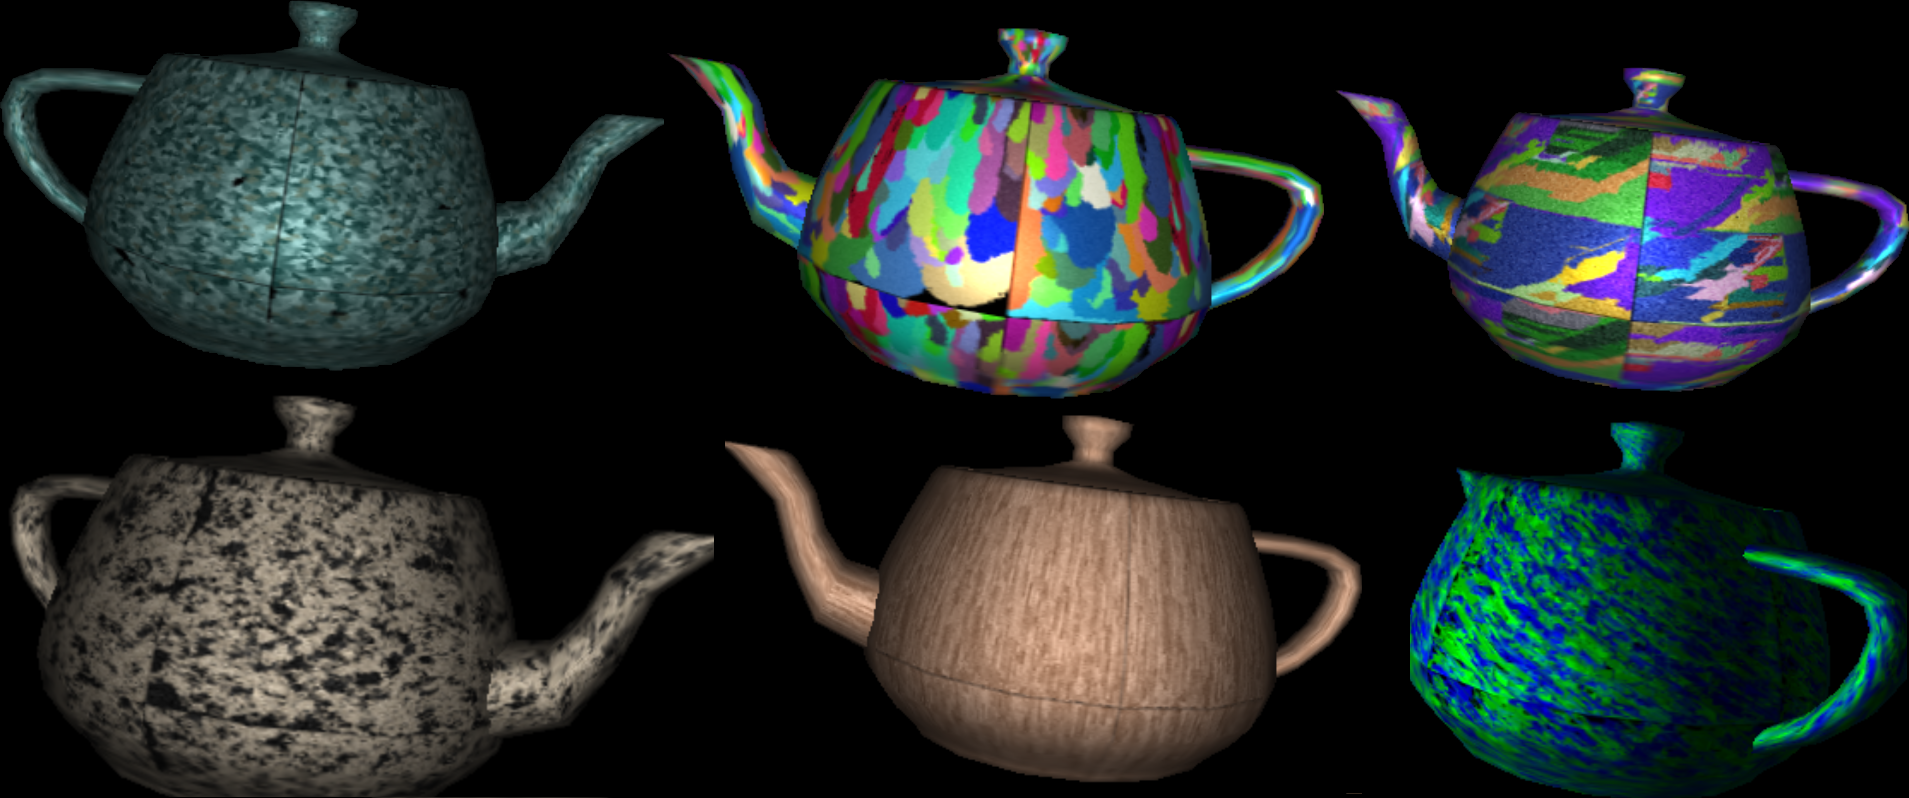
\includegraphics[scale=0.14]{figures/teteras}
\caption{Texturas generadas mapeadas en una tetera.}
\label{teteras}
\end{figure}


\begin{figure}[t!]
\centering
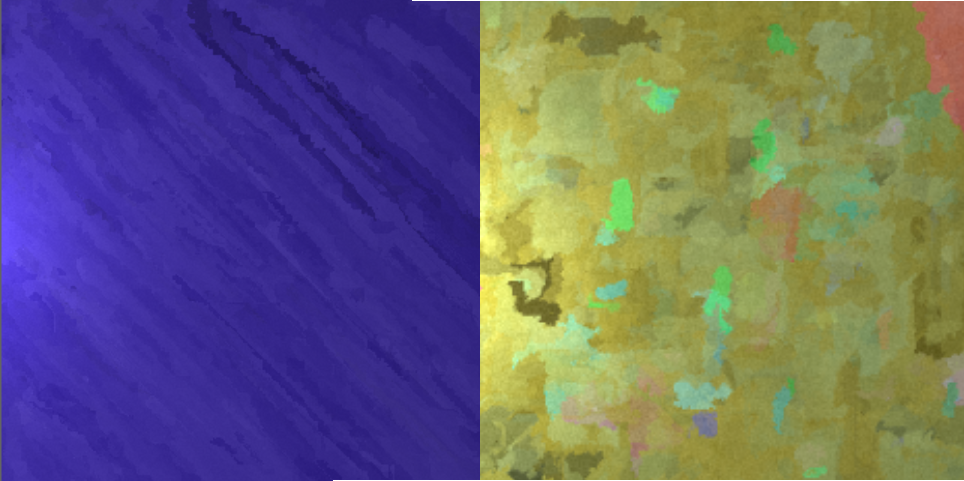
\includegraphics[scale=0.2]{figures/muerte}
\caption{Efecto producido utilizando el concepto de muerte de las partículas.}
\label{muerte}
\end{figure}

Los resultados obtenidos muestran una flexibilidad útil para producir distintos materiales.
Como fue aclarado, la idea de utilizar sistemas de partículas para producir materiales será utilizada en la sección siguiente.
Para esto, se generalizarán los resultados a tres dimensiones.

\section{Modelado Procedimental de Geometrías Porosas}

Utilizamos los sistemas de partículas previamente mencionados, en un cubo (tres dimensiones), pero reemplazando las direcciones de crecimiento por sistemas dinámicos \cite{Strogatz2001}, para hacer evolucionar las partículas dentro del sistema, produciendo patrones con formas geométricas naturales.
Este constituye un intento por simular, entre otros,  el efecto de la levadura en la masa cruda del pan.
Estos procedimientos producen distribuciones de burbujas de distintos tamaños, resultando en un mecanismo controlable, que presenta propiedades estadísticas.
Si bien la metodología introducida no está basada en primeros principios, la misma constituye un paso previo que permite sentar las bases de un modelo inspirado físicamente, el cual se presentará en la siguiente sección.

\subsection[Sistemas Dinámicos y Geometrías Porosas]{Sistemas Dinámicos como Modelo de Geometrías Porosas}
El propósito de este algoritmo constituye producir una textura volumétrica que representará una geometría, la cual se renderizará posteriormente.
Por lo tanto, en lugar de devolver el color de una posici\'on espec\'ifica, el algoritmo genera una textura volumétrica binaria, ceros y unos (cero si la posici\'on contiene aire, uno si la misma contiene masa).

Similarmente al caso de generación de texturas, el sistema consta de un conjunto de part\'iculas $P$,

\begin{equation}
  P = \{p_{1}, ... , p_{n}\}, n  \in \mathbb{N},
\end{equation}

\noindent dos grillas $L$ y $L^{2}$, donde la grilla $L_{N\times N \times N}, N \in \mathbb{N}$ (inicialmente $L_{xyz}=1$) representa masa y aire como fue descripto previamente, y $L^{2}_{N\times N \times N}$, (inicialmente $L^{2}_{xyz}=-1$) representa posiciones donde cada celda almacena un único entero, indicando qu\'e part\'icula adue\~na la misma ($i$ si el elemento de la grilla pertenece al contorno o interior de la part\'icula $i$).

Cada elemento en $P$ posee las siguientes propiedades:

\begin{equation}
  p_{i} = \{O_{i}, C_{i}\}, 1 \le i \le n,
\end{equation}

\noindent donde:

\begin{itemize}
\item $O_{i} = \{o_{1}, ... , o_{n_{i}}\}$: (Ocupadas) vector (conjunto) de posiciones ocupadas por la part\'icula en $L$.

\item $C_{i} = \{c_{1}, ... , c_{m_{i}}\}$: (Contorno) vector (conjunto) de posiciones representando el {\em contorno} de la part\'icula en $L$.
\end{itemize}

El vector $O$ representa las posiciones que ser\'an afectadas por la part\'icula, y el contorno $C$ se utiliza para asegurar que las part\'iculas se eviten entre s\'i.
El procedimiento se describe, simplificadamente, en el Algoritmo $1$. 

\begin{algorithm}[h!]
\caption{Algoritmo de modelado}
\begin{algorithmic}

\State{$t  = 0$}
\Comment{tiempo - iteración}
\State{$P  = []$}
\Comment{partículas}
\State{$L  = matriz(MxMxM).valores\_iniciales(1)$}
\Comment {Geometría - iniciada a 1 (masa)}
\State{$L^{2} = matriz(MxMxM).valores\_iniciales(-1)$}
\Comment{Dominio de cada partícula}

\For{$i \in [1,Cantidad\_Particulas]$}
    \Comment{Cada partícula toma una posición aleatoria en L}
    \State{$x \gets aleatorio, y \gets aleatorio()$}
    \State{$O[i] \gets [[x,y]]$}
    \State{$C[i] \gets []$}
    \For{$v \in vecindario(x,y)$}
        \State{$C[i].agregar(v)$}
    \EndFor
    \State{$P.agregar([O[i],C[i]])$}
\EndFor

\For {$t \in [0,tiempo\_max]$}
    \For {$i \in [1,Cantidad\_Particulas]$}
        \If {$vacio?~C[i]$}
            \State{morir()}
        \EndIf
        \For{$h \in C[i]$}
            \State{$C[i].eliminar(h)$}
            \Comment{la posición ya fue explorada}
            \State{// Si la pos. o contorno pertenecen a otra partícula, descartar}
            \State{// borde\_libre chequea disponibilidad en el vecindario}
            \If{$!(L^{2}[h] > 0 ~\&\&~ L^{2}[h] != i ~\&\&~ borde\_libre(separacion)$}
                \State{// Posición libre, ocupar}                
                \State{$L[h] \gets 0$} \Comment{masa -> aire}
                \State{$O[i].agregar(h)$}
                \State{$C[i].agregar(vecindario(h))$} 
                \State{$L^{2}.setear(vecindario(h),i)$} \Comment{Marcar posiciones en $L^{2}$ como $i$}
                \State{$L^{2}.setear(h,i)$}
                \Comment{turno de la particula $i+1$...}
            \EndIf
        \EndFor
    \EndFor
\EndFor
\end{algorithmic}
\end{algorithm}

Cuando $t = 0$, un conjunto de part\'iculas iniciales toman posiciones aleatorias en la textura volumétrica.
Para cada partícula, la posici\'on elegida resulta la primera ocupada en $O$, adem\'as, el vecindario de $O$ se agrega a $C$.
Cada part\'icula evoluciona en un intento por extender sus voxels ocupados ($O$), marcándolos en $L$. Los mismos se toman de $C$.
Cuando una part\'icula ocupa una entrada en la textura volumétrica, la misma se elimina de $C$ y se agrega a $O$.
Luego el vecindario de ese voxel se agrega a $C$ (es decir las posiciones que rodean inmediatamente a la entrada tomada).
Las grillas se actualizan de la siguiente manera: $L$ se setea a $0$ en la entrada y $L^{2}$ se setea con el valor $i$ en los voxels que se agregan a $C$. Las part\'iculas s\'olo pueden crecer si el valor encontrado en $L^{2}$ no pertenece a otra part\'icula.
El tama\~no del vecindario se par\'ametriza, definiendo la distancia entre part\'iculas.
Si el vector $C$ est\'a vac\'io, la part\'icula {\em muere} ya que no puede continuar creciendo.


El algoritmo puede ser terminado en cualquier $t$ deseado. El mismo puede finalizar su c\'omputo ante determinados eventos, por ejemplo, cuando todas las posiciones de $L^{2}$ fueron tomadas por part\'iculas, ya que no pueden realizarse progresos.

Variando el par\'ametro de distancia entre part\'iculas (separación) se obtienen distintas estructuras (ver Fig.~\ref{fg:sistdin1}). Las im\'agenes muestran ejemplos 2D (para mayor claridad) de crecimiento aleatorio de part\'iculas. La regi\'on blanca en las im\'agenes representa la masa restante luego del proceso.


\begin{figure*}[htb!]
  \centerline{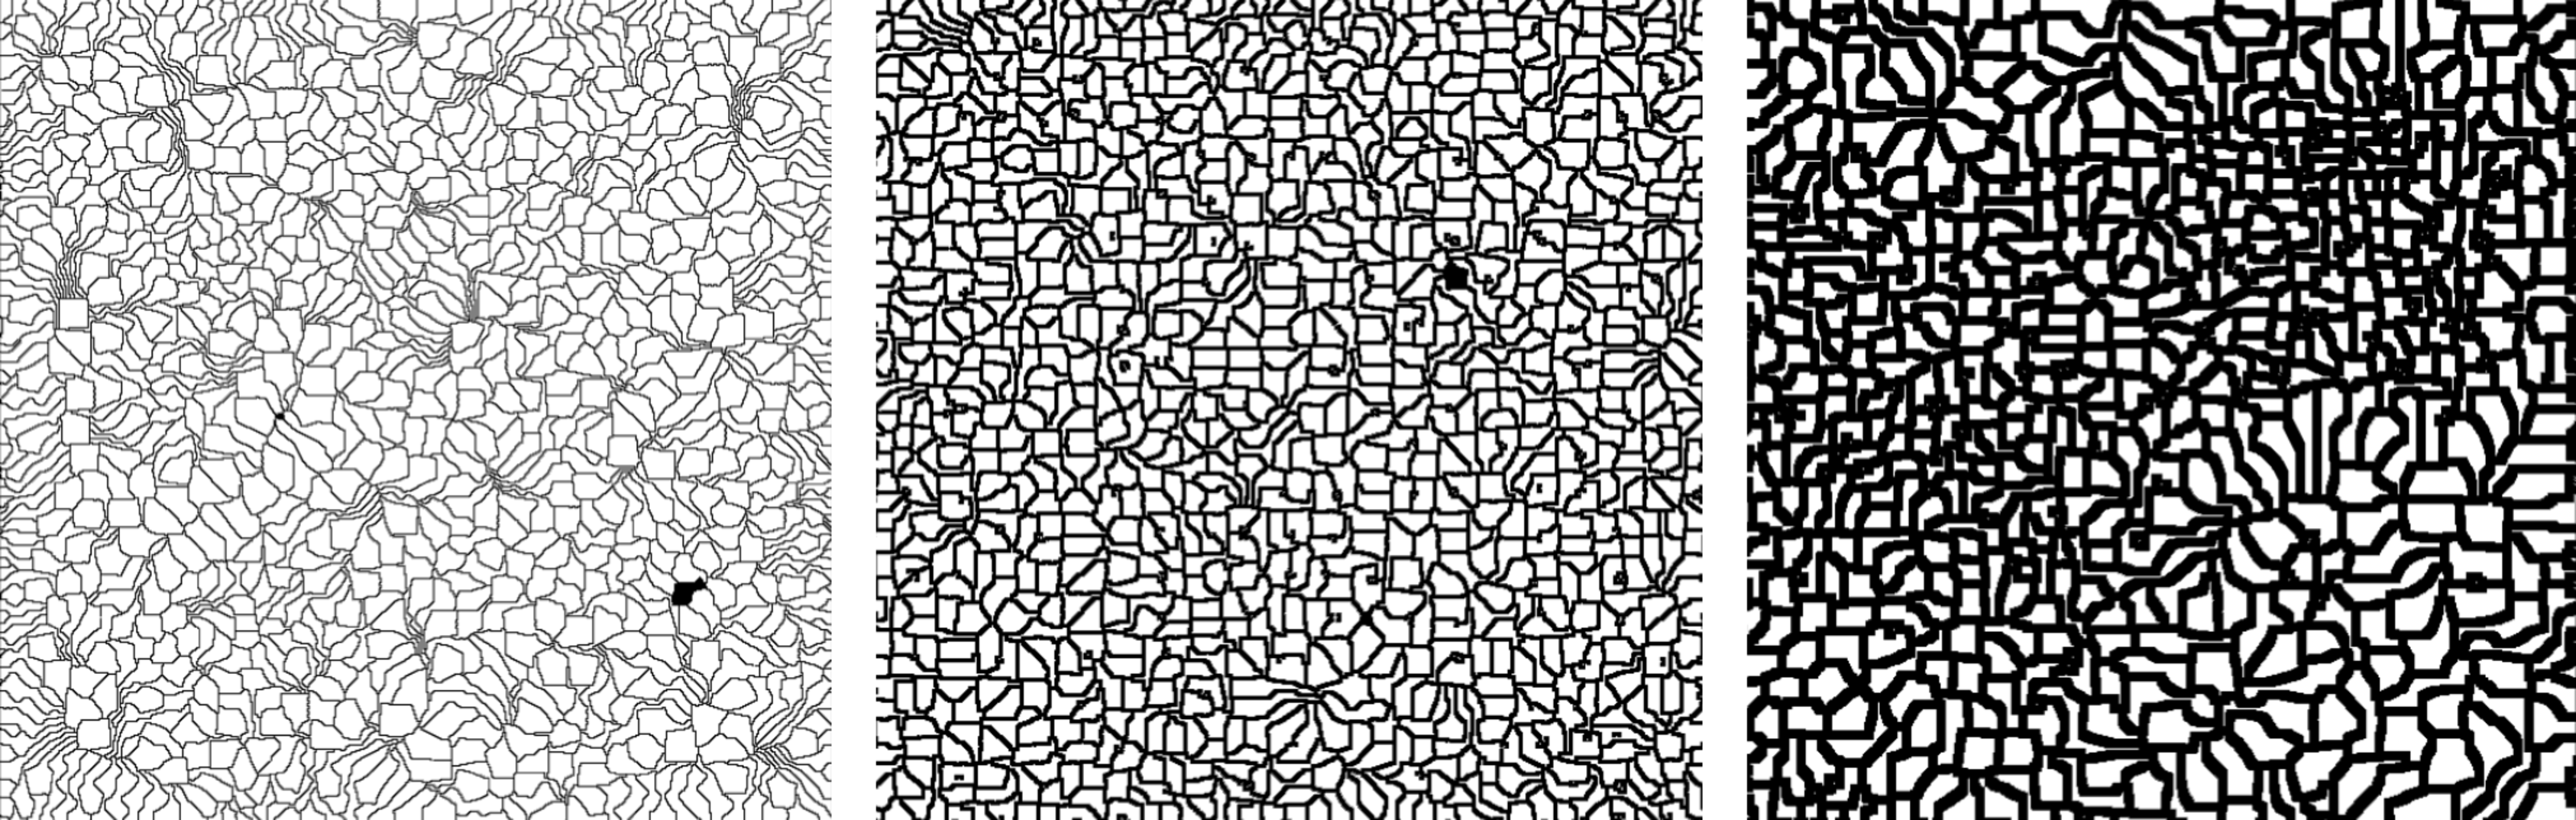
\includegraphics[width=13cm]{figures/Fig1}}
  \caption[Efecto del parámetro separación entre partículas.]{Efecto del parámetro separación entre partículas. Izquierda: separaci\'on = 1, centro: separaci\'on = 2, derecha: separaci\'on = 4.}
  \label{fg:sistdin1}
\end{figure*}

Finalmente, el algoritmo devuelve la grilla $L$, la cual ser\'a renderizada posteriormente. En la siguiente secci\'on se explica la utilizaci\'on de sistemas din\'amicos en la evoluci\'on guiada de part\'iculas.

\subsection{Sistemas Din\'amicos}

Las ecuaciones diferenciales tienen como prop\'osito tratar con la dificultad (o imposibilidad) de hallar soluciones anal\'iticas en procesos din\'amicos.
En primer lugar, se define un modelo matem\'atico del fenómeno, del cual luego se obtienen 
las ecuaciones diferenciales asociadas. Las mismas se resuelven por medio de aproximaciones num\'ericas en cada instante de tiempo.

Los costos computacionales de estas soluciones dependen de la complejidad del fenómeno y el n\'umero de ecuaciones del sistema. En este trabajo proponemos utilizar una sub-\'area de ecuaciones diferenciales llamada ecuaciones diferenciales ordinarias (ODE). En esta representaci\'on, el tiempo se trata como la \'unica variable independiente.


De manera general, las ODEs se representan utilizando el siguiente sistema de ecuaciones:
\begin{equation} \label{eq:simple}  
  \begin{aligned}
    \dot{x_{1}} = f_{1}(x_{1},\ldots,x_{n}),\\
    \ldots\\
    \dot{x_{n}} = f_{n}(x_{1},\ldots,x_{n}),
  \end{aligned}
\end{equation}

\noindent donde $\dot{x_{i}}$ representa la derivada de $x_{i}$ con respecto
a $t$.
Las variables $x_{i}$ y las funciones $f_{i}$ se definen de manera diferente en cada modelo.
En este caso, cada variable representa una coordenada cartesiana en el espacio, $x_{1}$ es $x$, $x_{2}$ es $y$ y $x_{3}$ es $z$.
El conjunto de $f_{i}$ ser\'a definido tratando de capturar la estructura interna del pan. 
La siguiente secci\'on muestra cómo estos sistemas pueden describir la evoluci\'on de los sistemas de part\'iculas.

\subsection{Evoluci\'on de sistemas de part\'iculas utilizando sistemas din\'amicos}

La percepci\'on humana puede detectar patrones en la estructura de la miga de pan. Distintas observaciones pueden realizarse sobre la distribuci\'on de las burbujas en la misma (ver Fig.~\ref{fg:panreal}).
Primero, la forma de las burbujas cercanas a la corteza tiende a estirarse paralelamente a la misma, como resultado de la acci\'on de las elevadas temperaturas durante la cocci\'on de la masa.
Tambi\'en resulta evidente que la estructura completa posee la apariencia de un fluido con la forma de la corteza.


\begin{figure*}[htb!]
  \centerline{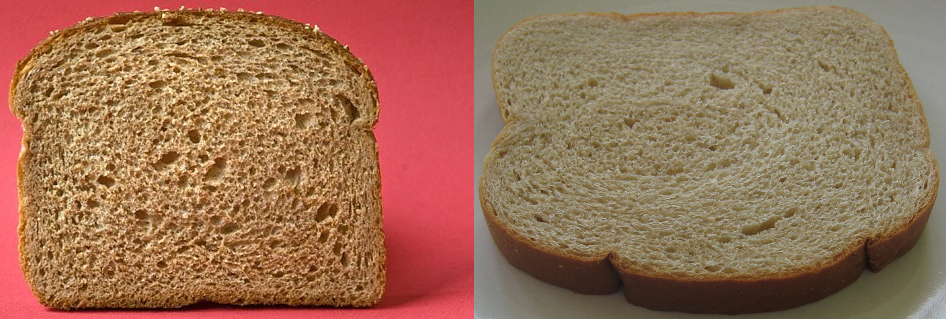
\includegraphics[width=13cm]{figures/panreal}}
  \caption[Imágenes de cortes reales de pan]{Imágenes de cortes reales de pan, obtenidas online\protect\footnotemark \protect\footnotemark  }
  \label{fg:panreal}
\end{figure*}

\footnotetext{http://jeremyrenners.blogspot.com.ar/2009/01/slice-of-bread.html}
\footnotetext{https://markforeman.wordpress.com/category/dehydration/}

Por otro lado, los sistemas din\'amicos previamente presentados producen formas naturales (ver Fig.~\ref{fg:sistdin2}).
En las im\'agenes pueden observarse c\'irculos y espirales, entre otras formas.
Las im\'agenes se obtuvieron dibujando trayectorias sobre un plano, siguiendo distintas ODEs.
Tres ODEs describen las din\'amicas presentes en las im\'agenes.
A modo de ejemplo, el siguiente conjunto de ecuaciones produce la imagen a la izquierda:

\begin{equation} \label{eq:simple}  
  \begin{aligned}
    \dot{x} &= x^{2}-y^{2}+1,\\
    \dot{y} &= 2xy+1.
  \end{aligned}
\end{equation}


\begin{figure*}[htb!]
  \centerline{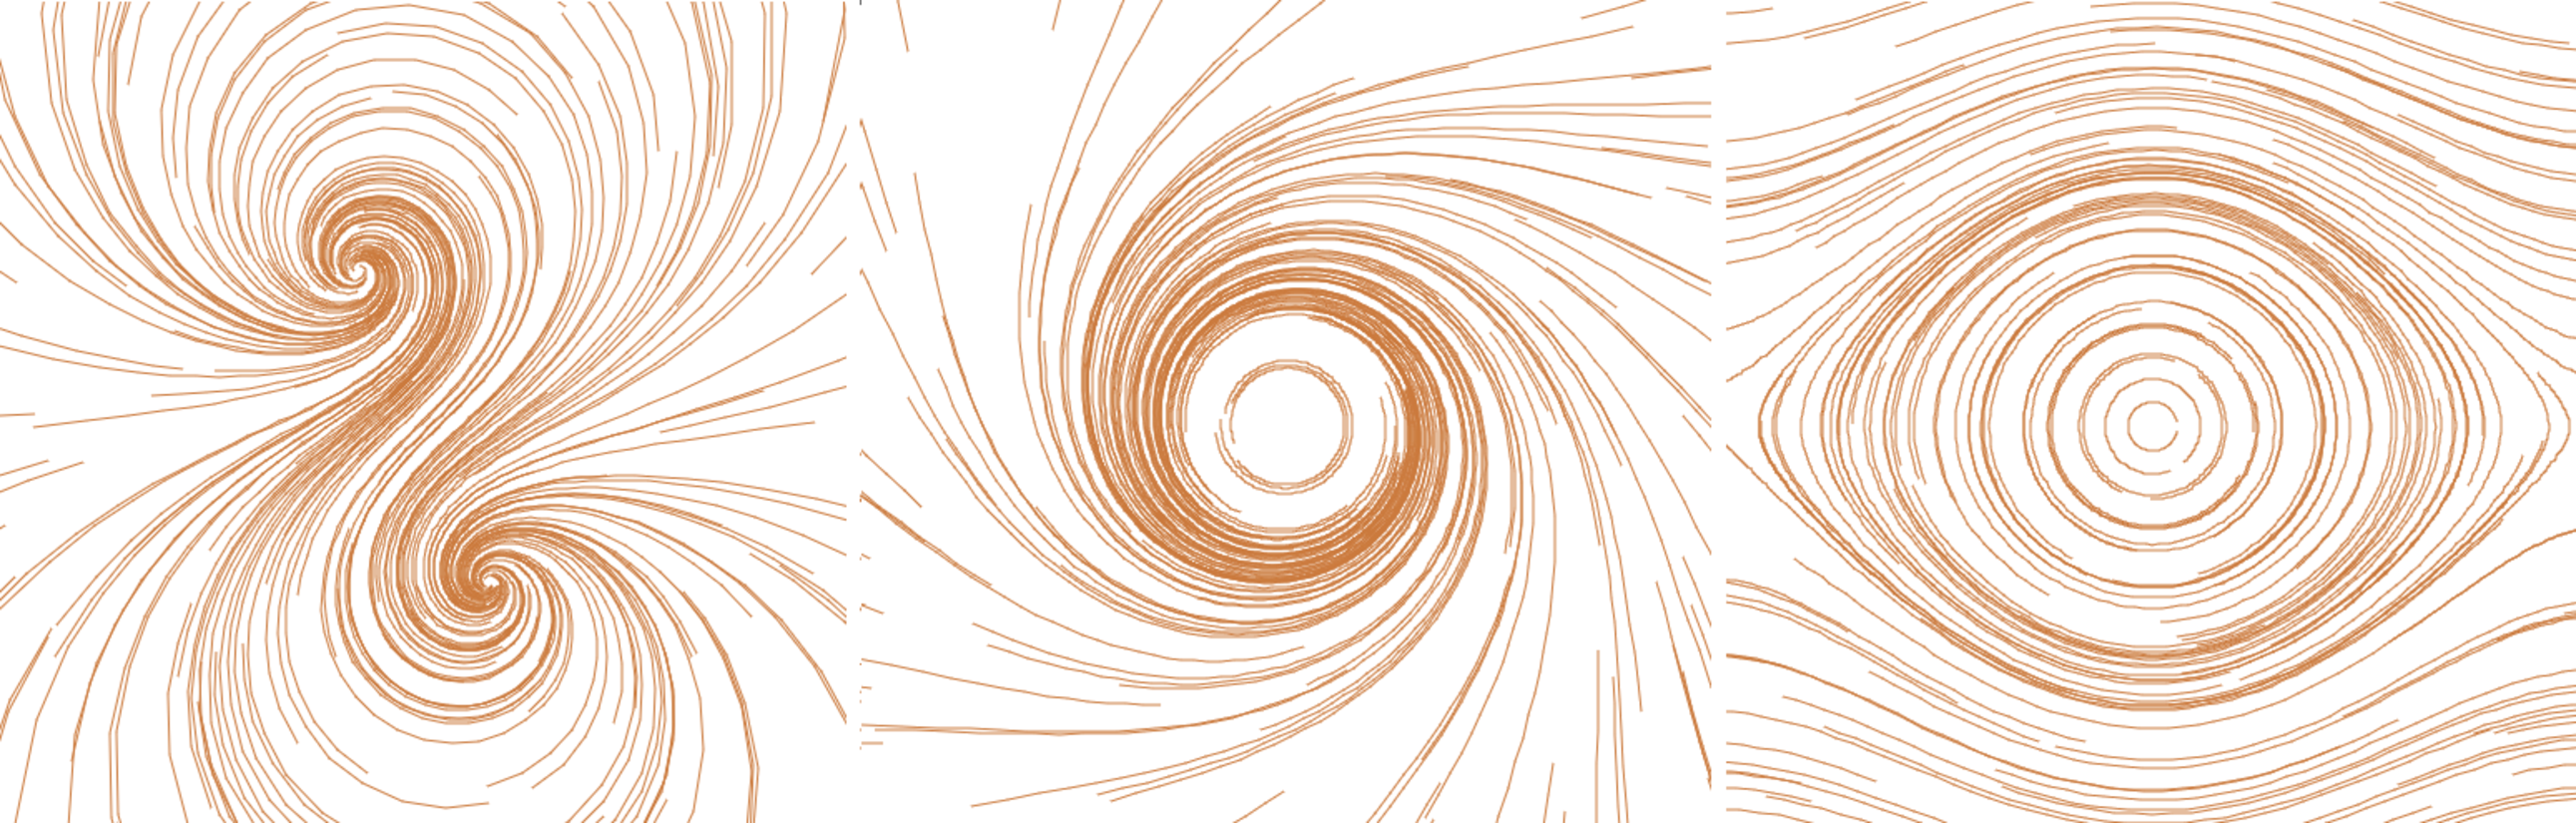
\includegraphics[width=13cm]{figures/Fig2}}
  \caption{Sistemas dinámicos en el plano.}
  \label{fg:sistdin2}
\end{figure*}

En los ejemplos se eligen posiciones aleatorias y luego el sistema se resuelve por medio de un {\em solver} Runge-Kutta de cuarto orden, el cual permite conocer la direcci\'on a tomar en cada punto por la trayectoria (en las im\'agenes se computaron trayectorias hacia adelante y hacia atrás en el tiempo para lograr una visualizaci\'on más clara).
La imagen de la izquierda muestra un atractor y un repeledor claramente visibles.
El centro de la espiral m\'as a la izquierda constituye un atractor (a medida que $t$ avanza, las trayectorias convergen hacia el punto), mientras que el otro centro representa un repeledor.
Los atractores pueden no ser puntuales, como muestran las restantes dos im\'agenes.
La imagen de la derecha muestra atractores en forma de c\'irculos (las trayectorias ciclan por el c\'irculo).

Las part\'iculas producen distintos patrones al seguir las trayectorias definidas en el plano y el espacio.
Esto se logra resolviendo num\'ericamente el sistema din\'amico en la posici\'on agregada a la part\'icula, seleccionando como siguiente posici\'on de crecimiento aquella posici\'on del contorno que aproxima con mayor precisión la soluci\'on del sistema din\'amico (para esto, sólo se agrega al contorno esa posición).
El Algoritmo $2$ muestra cómo se modifica el algoritmo de modelado para incluir este comportamiento.

\begin{algorithm}[h!]
\caption{Modificación del algoritmo de modelado por medio de sistemas dinámicos}
\begin{algorithmic}
\State $L[h]\gets 0$ \Comment{masa $\rightarrow$ aire}
\State $O[i].agregar(h)$
\State $solucion \gets Runge\_Kutta(h)$
\Comment {Se calcula la siguiente posición}
\State $vec = vecindario(h)$
\State $mejor = abs(vec[0] - solucion)$
\State $elegida = h$
\State $vec.eliminar(h)$
\For {$w \in vec$}
\State{// Se calcula la posición del vecindario que mejor aproxima al sistema}
    \If {$abs(vec[w]-solucion) < mejor$}
        \State $mejor = abs(vec[w]-solucion)$
        \State $elegida = w$
    \EndIf
    \If {$aleatorio() > 1-aleatoriedad$} 
    \Comment {$0 <= aleatorio() <= 1$}
        \State $C[i].agregar(w)$
    \EndIf
\EndFor
\State{// Se agrega al vecindario sólo la posición que mejor aproxima la solución}
\State $C[i].agregar(elegida)$
\end{algorithmic}
\end{algorithm}

Las part\'iculas se deforman globalmente en un patr\'on visualmente similar a las trayectorias que produce el sistema (ver Fig.~\ref{fg:sistdin3}).
En las im\'agenes, de izquierda a derecha se decrementa la {\em aleatoriedad} de las trayectorias.
El par\'ametro aleatoriedad seteado a $0.1$ genera la imagen de la derecha, lo cual significa que las burbujas eligen como siguiente posición de crecimiento la que mejor se acopla al sistema con una probabilidad de $0.9$.
La probabilidad se define como $1-aleatoriedad$, donde $0 \leq aleatoriedad \leq 1$.
Las ecuaciones del sistema son las mismas que las de la imagen derecha mostrada en la Fig.~\ref{fg:sistdin2}.

\begin{figure*}[htb!]
  \centerline{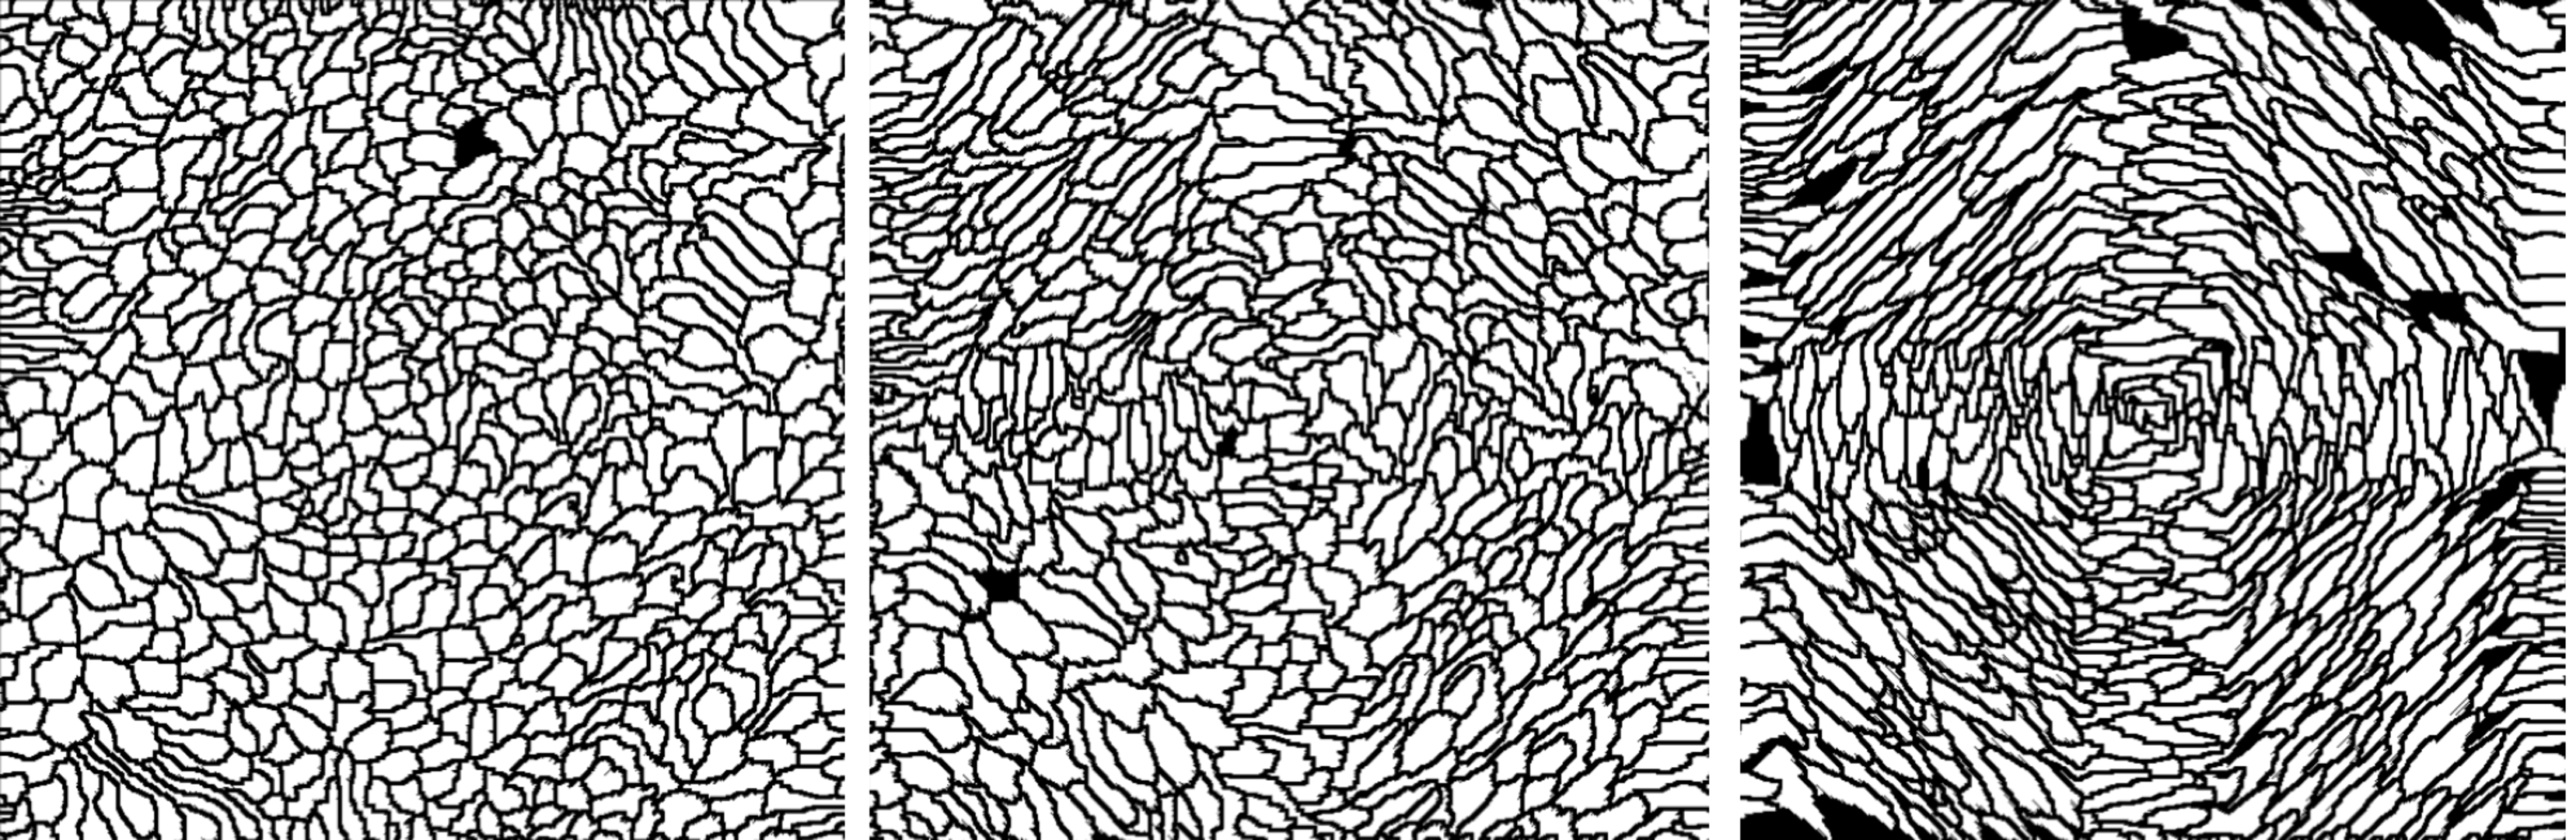
\includegraphics[width=13cm]{figures/Fig3}}
  \caption[Sistemas din\'amicos aplicados en sistemas de part\'iculas]{Sistemas din\'amicos aplicados en sistemas de part\'iculas. Efecto del parámetro {\em aleatoriedad}. De izquierda a derecha, aleatoriedad: 0.3,0.2,0.1 respectivamente. }
  \label{fg:sistdin3}
\end{figure*}

\subsection{Condiciones de contorno}
A partir de una geometría tridimensional dada, se establecen condiciones de contorno que las burbujas deben respetar durante su crecimiento.
Esto permite representar más fielmente estructuras porosas como huesos, panes y esponjas, dado que de esta forma las burbujas pueden realizar una interacción más realista con el contorno de los objetos.
Determinados materiales como huesos humanos o el pan presentan burbujas orientadas de manera paralela a las paredes del objeto, ya que durante el proceso de formación del material las burbujas son presionadas contra las paredes del mismo.
Huesos típicos presentan estructuas porosas y no porosas combinadas, y regiones donde el tejido trabecular (poroso) muestra una orientación definida en determinadas direcciones, dependiendo del estado de salud del hueso, la edad de la persona y otros factores.
En otras estructuras porosas como las esponjas, las celdas visibles en la estructura no presentan una orientación definida.

Nuestro modelo puede adaptarse a estas variadas situaciones definiendo sistemas dinámicos que varían de acuerdo a la región del material en la cual se encuentran.

El procedimiento comienza voxelizando una geometría de entrada arbitraria, definiendo una región de interés donde las partículas pueden crecer (seteando 1 si el voxel pertenece a la geometría, y 0 en otro caso).
Luego, definimos condiciones de contorno en la textura volumétrica resultante.
Para esto utilizamos un método por cortes bidimensionales de la textura, es decir, el sistema dinámico y su condición de borde se definen en un corte del volumen únicamente.
Si bien esto no resulta una parametrización 3D completa, la elección produce un algoritmo de modelado que es más intuitivo para definir y visualizar, ya que el sistema dinámico sólo necesita ser especificado en coordenadas 2D.

Para esto, se define un eje principal en el volumen entre los tres ejes Cartesianos (este eje resulta un parámetro del modelo), a partir del cual cada corte queda definido.
De cada corte obtenemos el centro de masa del mismo, estableciéndolo como centro.
Esto quiere decir que se define un patrón circular, inducido por el sistema dinámico, alrededor del mismo.
El sistema dinámico exacto puede variar, obteniendo apariencias ligeramente diferentes (espiral, círculo concéntrico, etc.).

Luego de que se eligió un eje principal, el procedimiento computa las condiciones de borde para cada voxel en el corte.
Para obtener estos valores, se computa un suavizado (utilizando filtrado gaussiano) de cada corte $s_{i}$.
El gradiente de este suavizado permite definir vectores gradientes en cada punto del borde de la geometría:

$$\displaystyle (v_{x},v_{y}) = g_{s_{i}}[x,y],$$

\noindent donde $v_{x}$ y $v_{y}$ son los componentes del vector gradiente en $x$ e $y$, respectivamente.
Un vector ortogonal a este puede utilizarse para seguir la silueta exterior del corte, y por lo tanto del volumen.
Para esto se computa el vector $(v_{y},-v_{x})$.
La Fig.~\ref{fg:Fig4} muestra el resultado de estos cómputos en un corte de una geometría.
El campo vectorial resultante sigue adecuadamente la forma exterior del corte.
La imagen también muestra que el método funciona en cortes con regiones desconectadas.


\begin{figure}
  \centerline{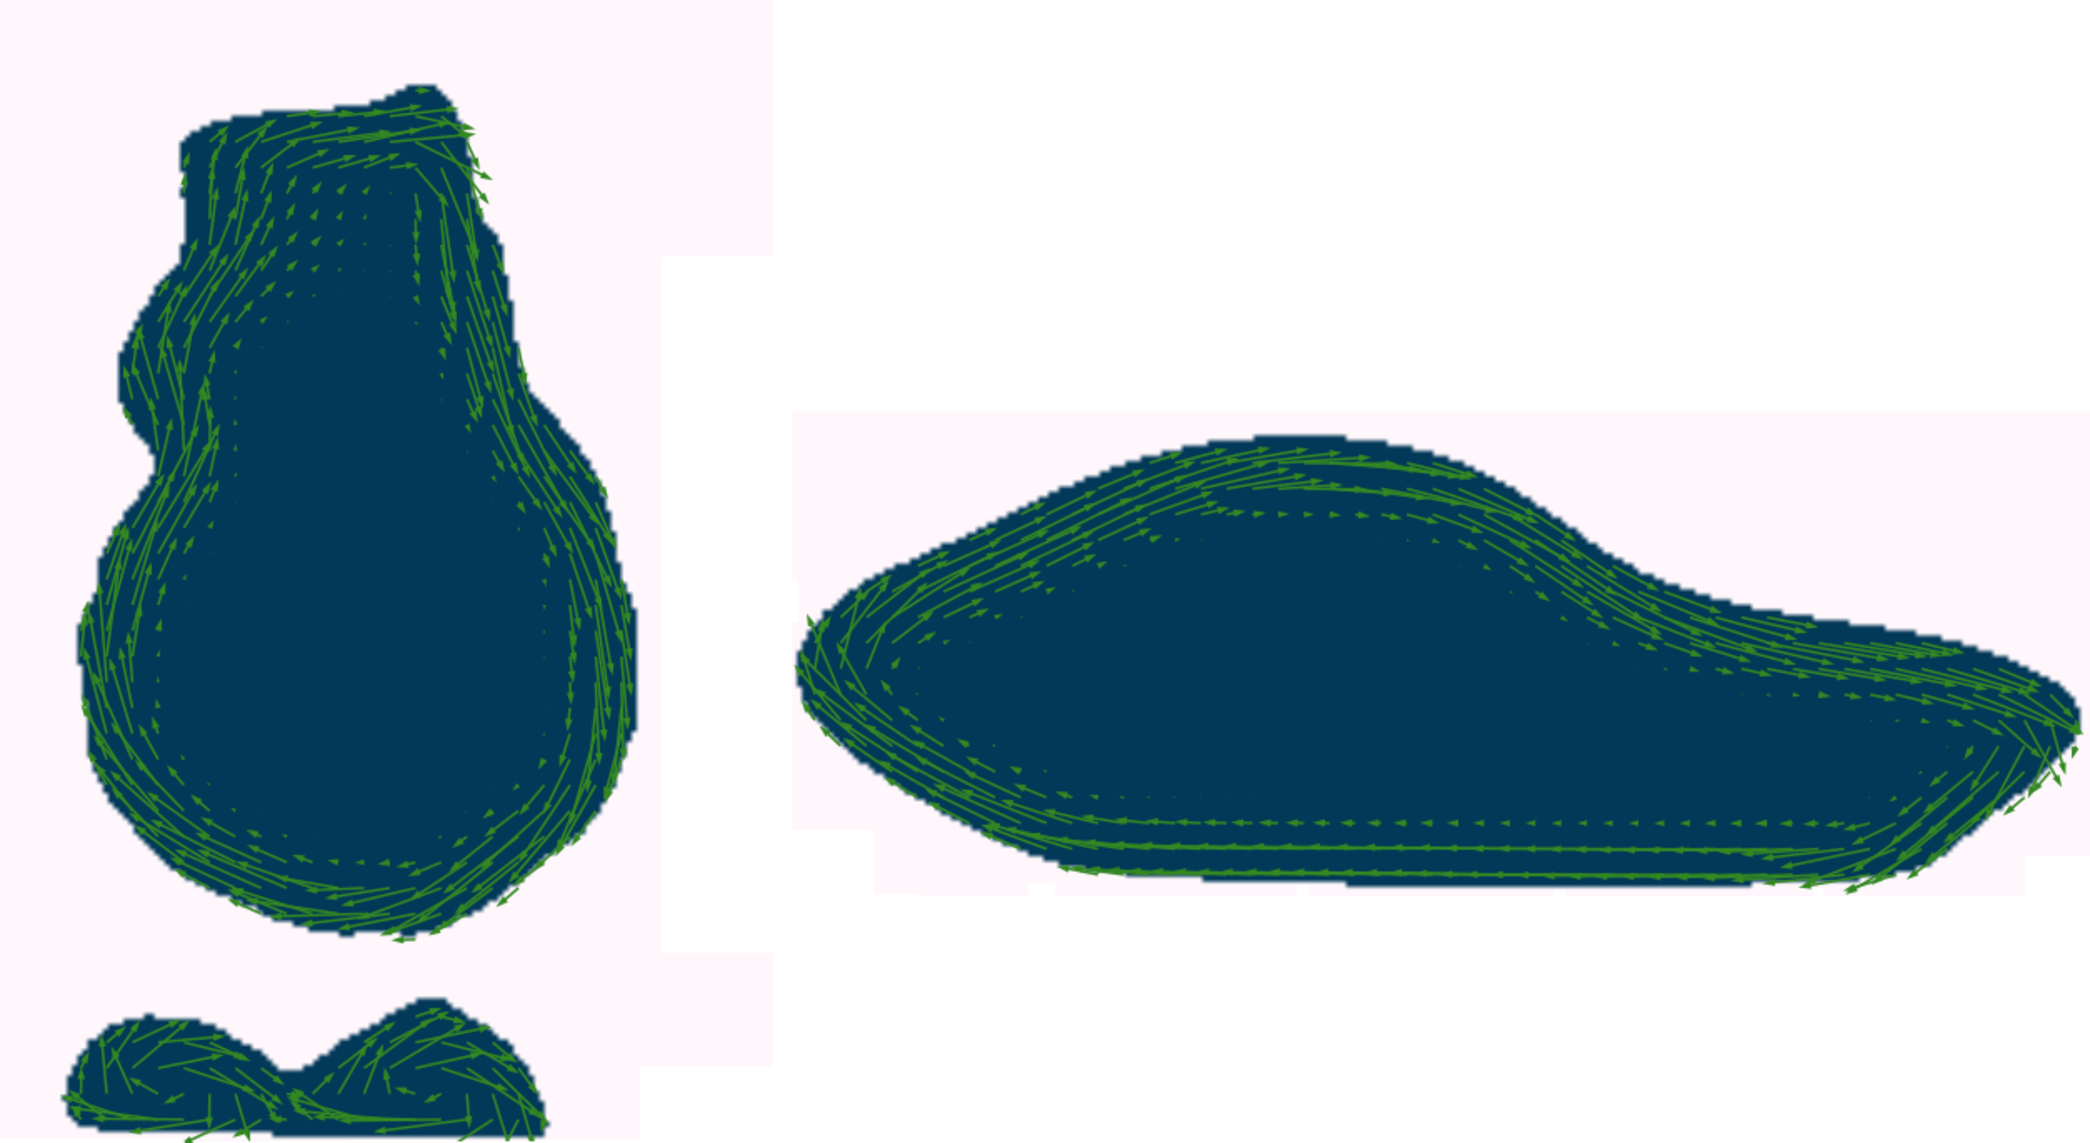
\includegraphics[width=11cm]{figures/Fig4}}
  \caption{Campo discreto de vectores perpendiculares al gradiente. La imagen muestra que los vectores computados siguen la silueta exterior de figuras arbitrarias. Por claridad solo se muestran algunos vectores del campo.}
  \label{fg:Fig4}
\end{figure}

Las condiciones de contorno se eligen si $v_{x}$ o $v_{y}$ resultan $>0$, caso contrario un sistema dinámico regula el crecimiento en el interior del corte bidimensional.
Este proceso crea un patrón global realístico de deformación en el corte, ver Fig.~\ref{fg:Fig5}.

Las burbujas tienden a permanecer en el corte bidimensional en el cual se originaron, pero debido al cómputo de números aleatorios en el proceso de crecimiento, las mismas no se limitan al corte mencionado, pudiendo cambiar entonces de corte y sistema dinámico.

\begin{figure}
  \centerline{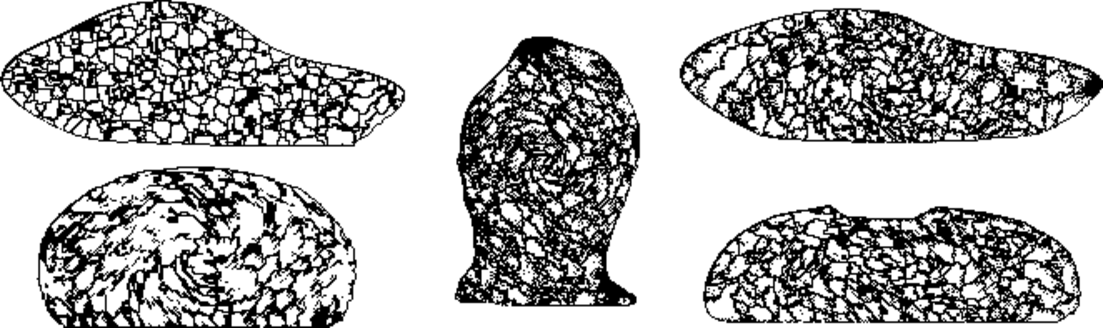
\includegraphics[width=15cm]{figures/Fig5}}
  \caption{Cortes porosos generados con el algoritmo de crecimiento propuesto. La imagen muestra que las burbujas siguen las condiciones de contorno cerca de los bordes de las geometrías y el sistema dinámico en el centro, produciendo patrones naturales tanto locales como globales. La imagen de la izquierda, arriba, utiliza un valor de aleatoriedad superior a las otras imágenes, produciendo una estructura parecida a una esponja. La imagen de la izquierda, abajo fue producida con el menor valor de aleatoriedad de todas las imágenes.}
  \label{fg:Fig5}
\end{figure}

El parámetro {\em aleatoriedad} puede utilizarse para determinar la homogeneidad de la textura resultante.
Por ejemplo, un valor cercano a 0 fuerza a las burbujas a seguir ajustadamente el sistema, lo cual es útil para determinados tipos de panes.
Un valor más alto del parámetro es útil para esponjas.

Adicionalmente, el método puede definir comportamiento diferente en distintas regiones, definiendo un sistema dinámico distinto para cada conjunto de cortes.
De esta forma la estructura porosa resultante podrá mostrar diferentes orientaciones dependiendo del voxel y el corte en el cual se observe.
Por ejemplo, es posible definir sistemas dinámicos que tomen en consideradión el ancho y alto del corte, produciendo burbujas que se adapten a esta situación: si el ancho es mayor al alto, se puede definir un sistema dinámico donde las burbujas crezcan horizontalmente.
Ídem si el alto es mayor que el ancho.
Un valor umbral relacionando el ancho y el alto puede definir cuándo se utilizan estos comportamientos.
La Fig.~\ref{fg:Fig6} muestra estas consideraciones.


\begin{figure}
  \centerline{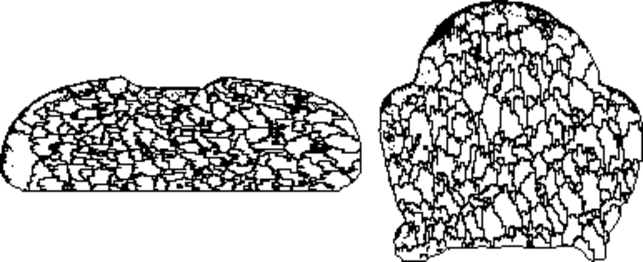
\includegraphics[width=11cm]{figures/Fig6}}
  \caption{Cortes 2D generados con sistemas dinámicos predominantemente horizontal (izquierda) y vertical (derecha). La imagen muestra que las burbujas resultantes producen patrones que se adaptan a la relación entre el ancho y el alto de cada corte.}
  \label{fg:Fig6}
\end{figure}


Como un ejemplo final, en la Fig.~\ref{fg:Fig7} se muestran cortes con forma de conejo, donde las burbujas ciclan sobre el centro de masa, y el parámetro {\em separación} es $2$.
Este ejemplo demuestra que el sistema puede ser configurado para atender a distintas configuraciones visibles en distintos materiales (en este caso al distancia entre las burbujas).


\begin{figure}
  \centerline{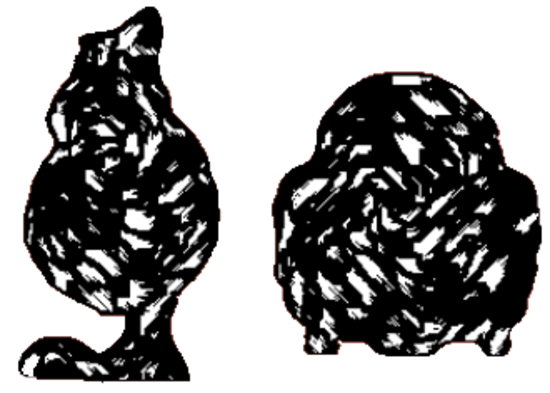
\includegraphics[width=9cm]{figures/Fig7}}
  \caption{Cortes con forma de conejo, donde las burbujas ciclan sobre el centro de masa del mismo. Adicionalmente, el parámetro {\em separación} es $2$.}
  \label{fg:Fig7}
\end{figure}

\subsection{Comparación con modelos de ruidos}
La generación artística de estructuras porosas es llevada a cabo usualmente utilizando distintos modelos de ruido, como ruido blanco, ruido Voronoi, ruido de Perlin \cite{Perlin1985}, y ruido de Worley \cite{Worley1996}.
Estos modelos generan poros por medio de variaciones aleatorias de valores, y posterior suavizado del volumen resultante.
Estos procedimientos arrojan resultados aceptables cuando los patrones finales no necesitan ser completamente controlados, dada la naturaleza aleatoria de los métodos.

En particular, el ruido blanco no captura la mesoestructura requerida para representar adecuadamente materiales porosos, debido a que la textura generada es muy poco realista.
De manera similar, el ruido de Perlin produce resultados muy suaves, con patrones estadísticos que inhabilitan la formación de poros de manera flexible, ver Fig.~\ref{fg:Fig8}.
Ambos modelos de ruido presentas dificultades para controlar el tamaño y la distribución resultante de poros.

Los ruidos de Voronoi y Worley son capaces de representar poros y sus distribuciones en posiciones arbitrarias en el espacio tridimensional.
Luego, se pueden definir funciones de distancia sobre estos puntos para construir densidades volumétricas, generando volúmenes de aire/masa.
Esto puede generar representaciones aceptables para esponjas y otros materiales homogéneos o con características aleatorias, como piedras y células.
Sin embargo, es muy difícil o muy {\em ad-hoc} obtener orientaciones específicas sobre los patrones resultantes, ver Fig.~\ref{fg:Fig9}.
Generalmente se requieren otras técnicas como mapas de texturas\footnote{https://graphics.stanford.edu/wikis/cs348b-11/aharaux/FinalProject} para obtener deformación de burbujas.

Nuestro procedimiento no requiere técnicas auxiliares para obtener patrones convincentes, debido a que el sistema dinámico captura la dinámica de estos comportamientos.
Esto implica que nuestro método reduce tiempo y complejidad en el modelo.
El método resultante es altamente parametrizable y completamente automático, permitiendo utilizar la técnica no sólo a programadores y expertos en computación gráfica, sino también a artistas.


\begin{figure}
  \centerline{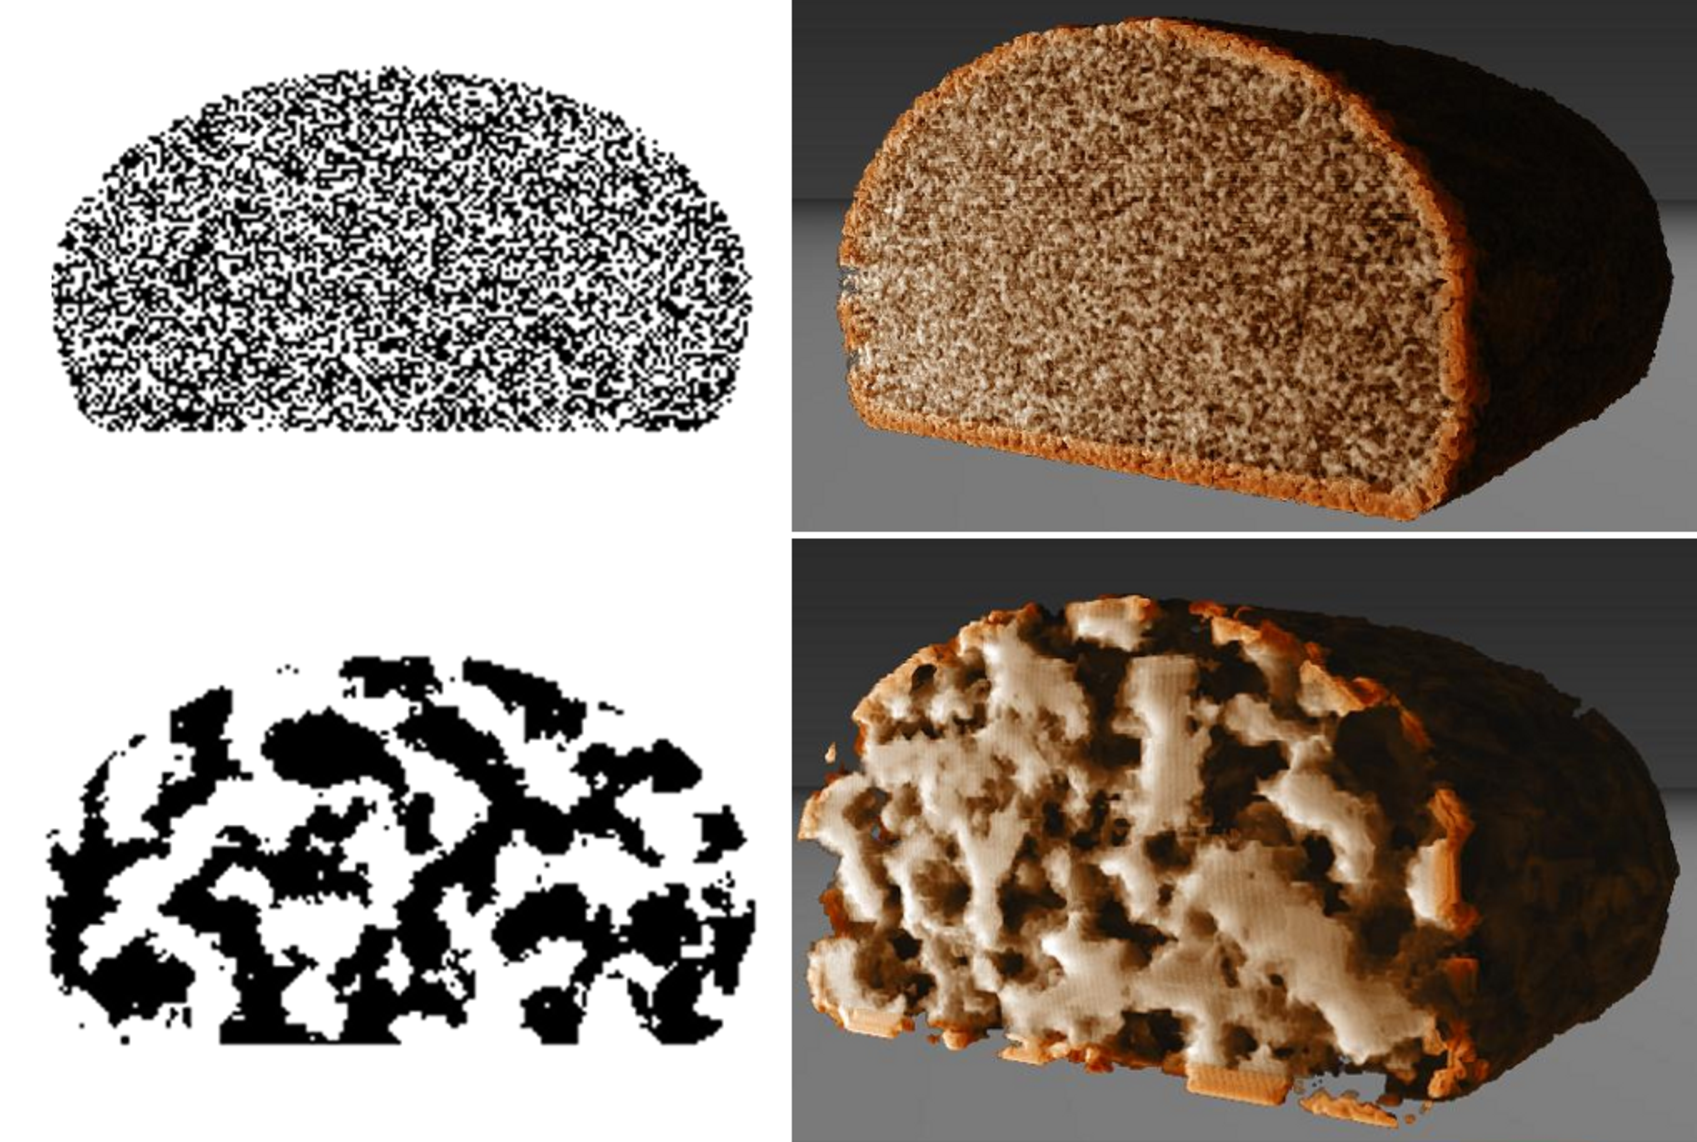
\includegraphics[width=11cm]{figures/Fig8}}
  \caption{Estructura porosa simulada con ruido blanco (arriba) y ruido de Perlin (abajo). La imagen muestra que el material no es poroso (arriba) o es demasiado suave (abajo), haciendo difícil controlar las posiciones y la distribución de tamaños de poros.}
  \label{fg:Fig8}
\end{figure}

\clearpage

\begin{figure}
  \centerline{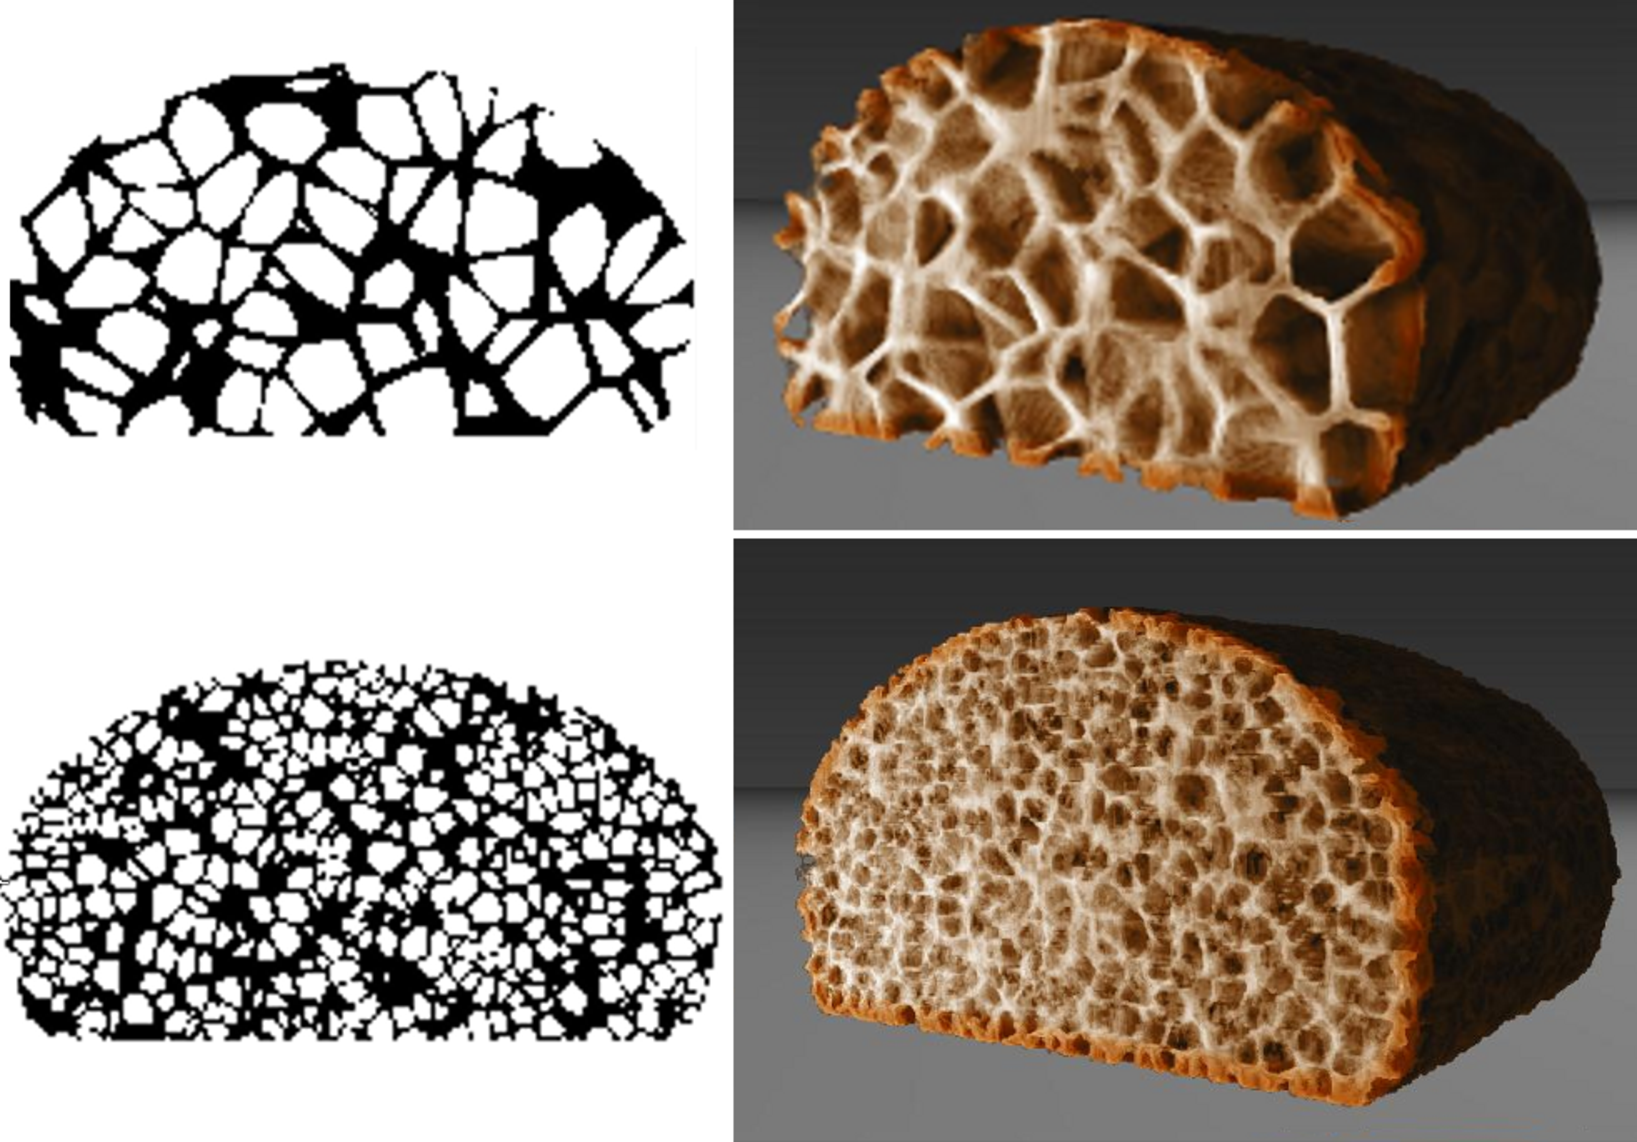
\includegraphics[width=11cm]{figures/Fig9CAVW}}
  \caption{Estructura porosa simulada con ruido de Voronoi (arriba) y ruido de Worley (abajo). La imagen muestra que si bien los métodos generan estructuras porosas convincentes, los usuarios de las mismas deben emplear técnicas auxiliares para obtener flexibilidad en los patrones resultantes (por ejemplo para controlar la orientación y forma de los poros).}
  \label{fg:Fig9}
\end{figure}

\subsection{Resultados y Limitaciones}
En las Figs.~\ref{fg:Fig11} y \ref{fg:Fig12} se muestran imágenes sintetizadas a través del procedimiento de partículas descrito, utilizando el método de renderizado del siguiente capítulo.
Las imágenes muestran objetos cuyo materiales se asemejan a panes, tanto en apariencia como en los patrones de sus burbujas.
Las Figs.~\ref{fg:Fig13} y \ref{fg:Fig14} se muestran esponjas y piedras porosas sintetizadas con el mismo procedimiento, utilizando distintos valores para la aleatoriedad y la cantidad de burbujas iniciales.
La Fig.~\ref{fg:Fig11} resalta el resultado de utilizar poca aleatoriedad en el crecimiento de las burbujas, forzando a las mismas a seguir un sistema dinámico circular.
Estos patrones pueden ser utilizados adem\'as en otros materiales cocidos, variando el par\'ametro de aleatoriedad.
Si bien es posible generar distintas geometrías de manera sencilla y automática, se requiere mayor profundidad en la investigación para determinar sistemas adecuados para determinados materiales.
Los resultados alcanzados permiten obtener buenos resultados para panes, esponjas, y piedras, como fue mostrado, entre otros.
Sin embargo, para posibilitar una renderización convincente de materiales como huesos debe extenderse el método para atender a las necesidades específicas del material, dado que en el mismo los patrones no son completamente aleatorios, y determinadas zonas presentan orientaciones claramente definidas en muestras reales.

\begin{figure}
  \centerline{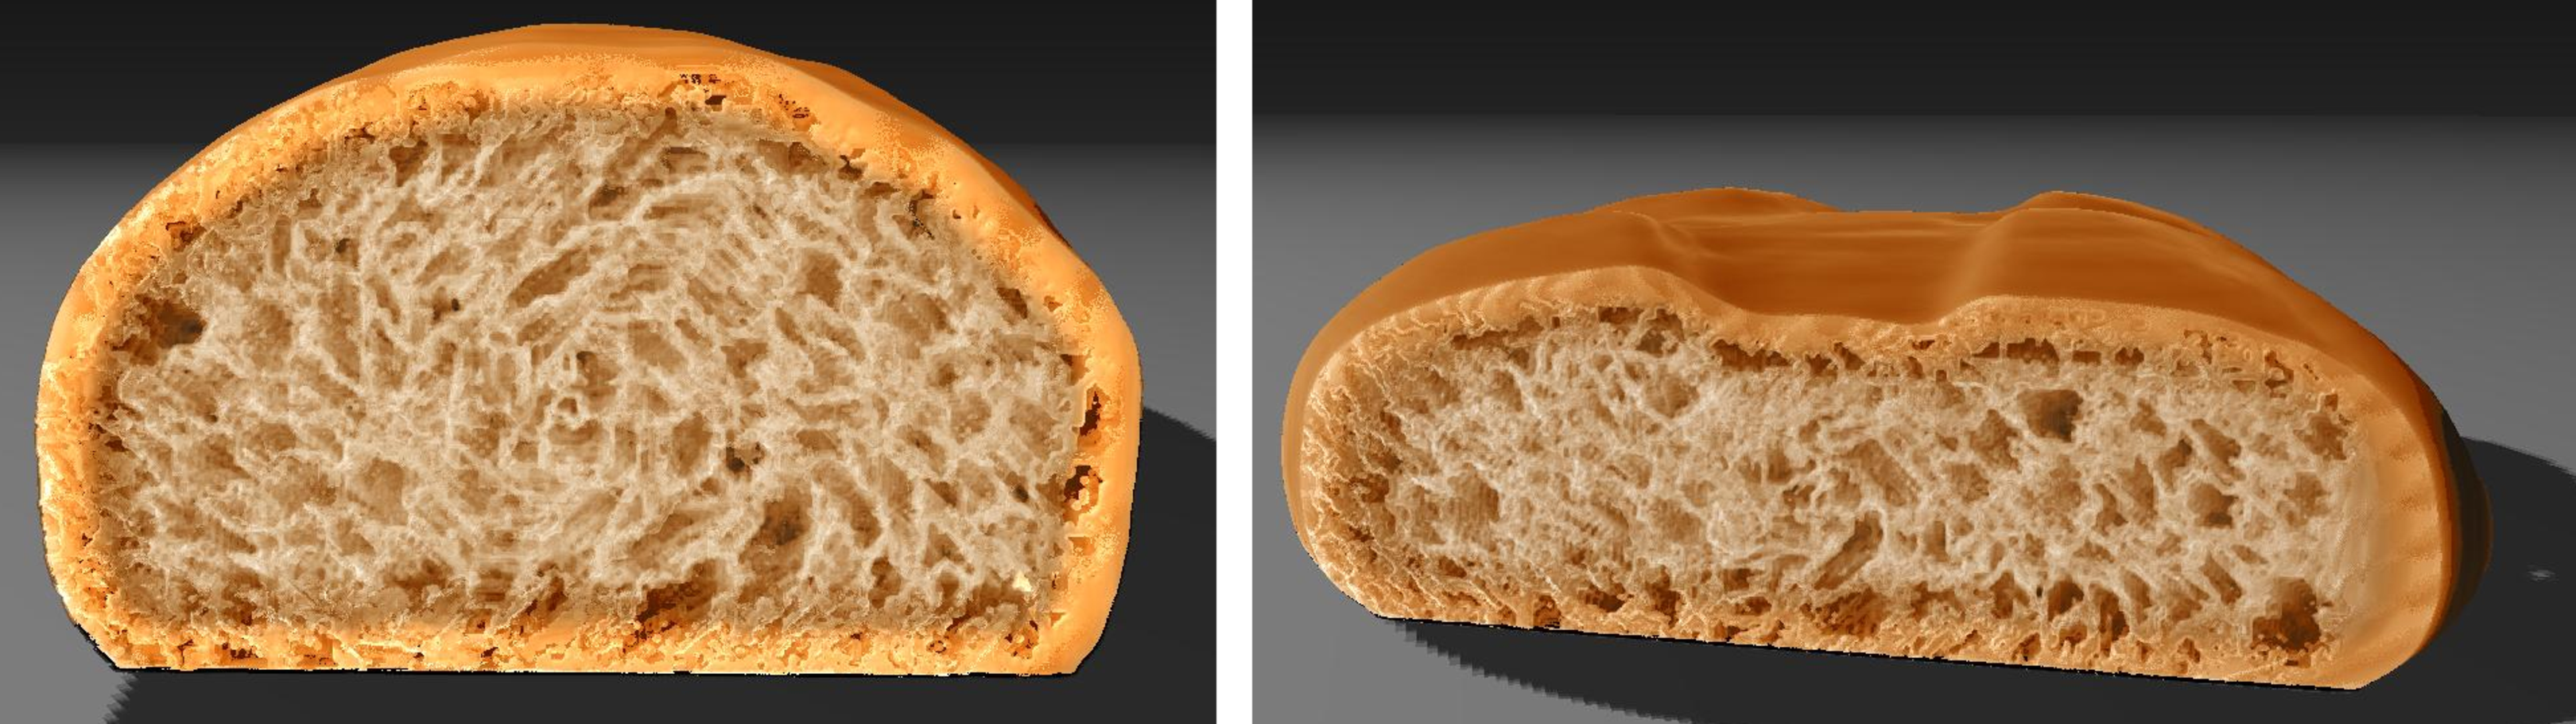
\includegraphics[width=12cm]{figures/Fig11CAVW}}
  \caption{Panes renderizados, destacando burbujas concéntricas sobre el centro de masa de cada corte bidimensional.}
  \label{fg:Fig11}
\end{figure}

\begin{figure}
  \centerline{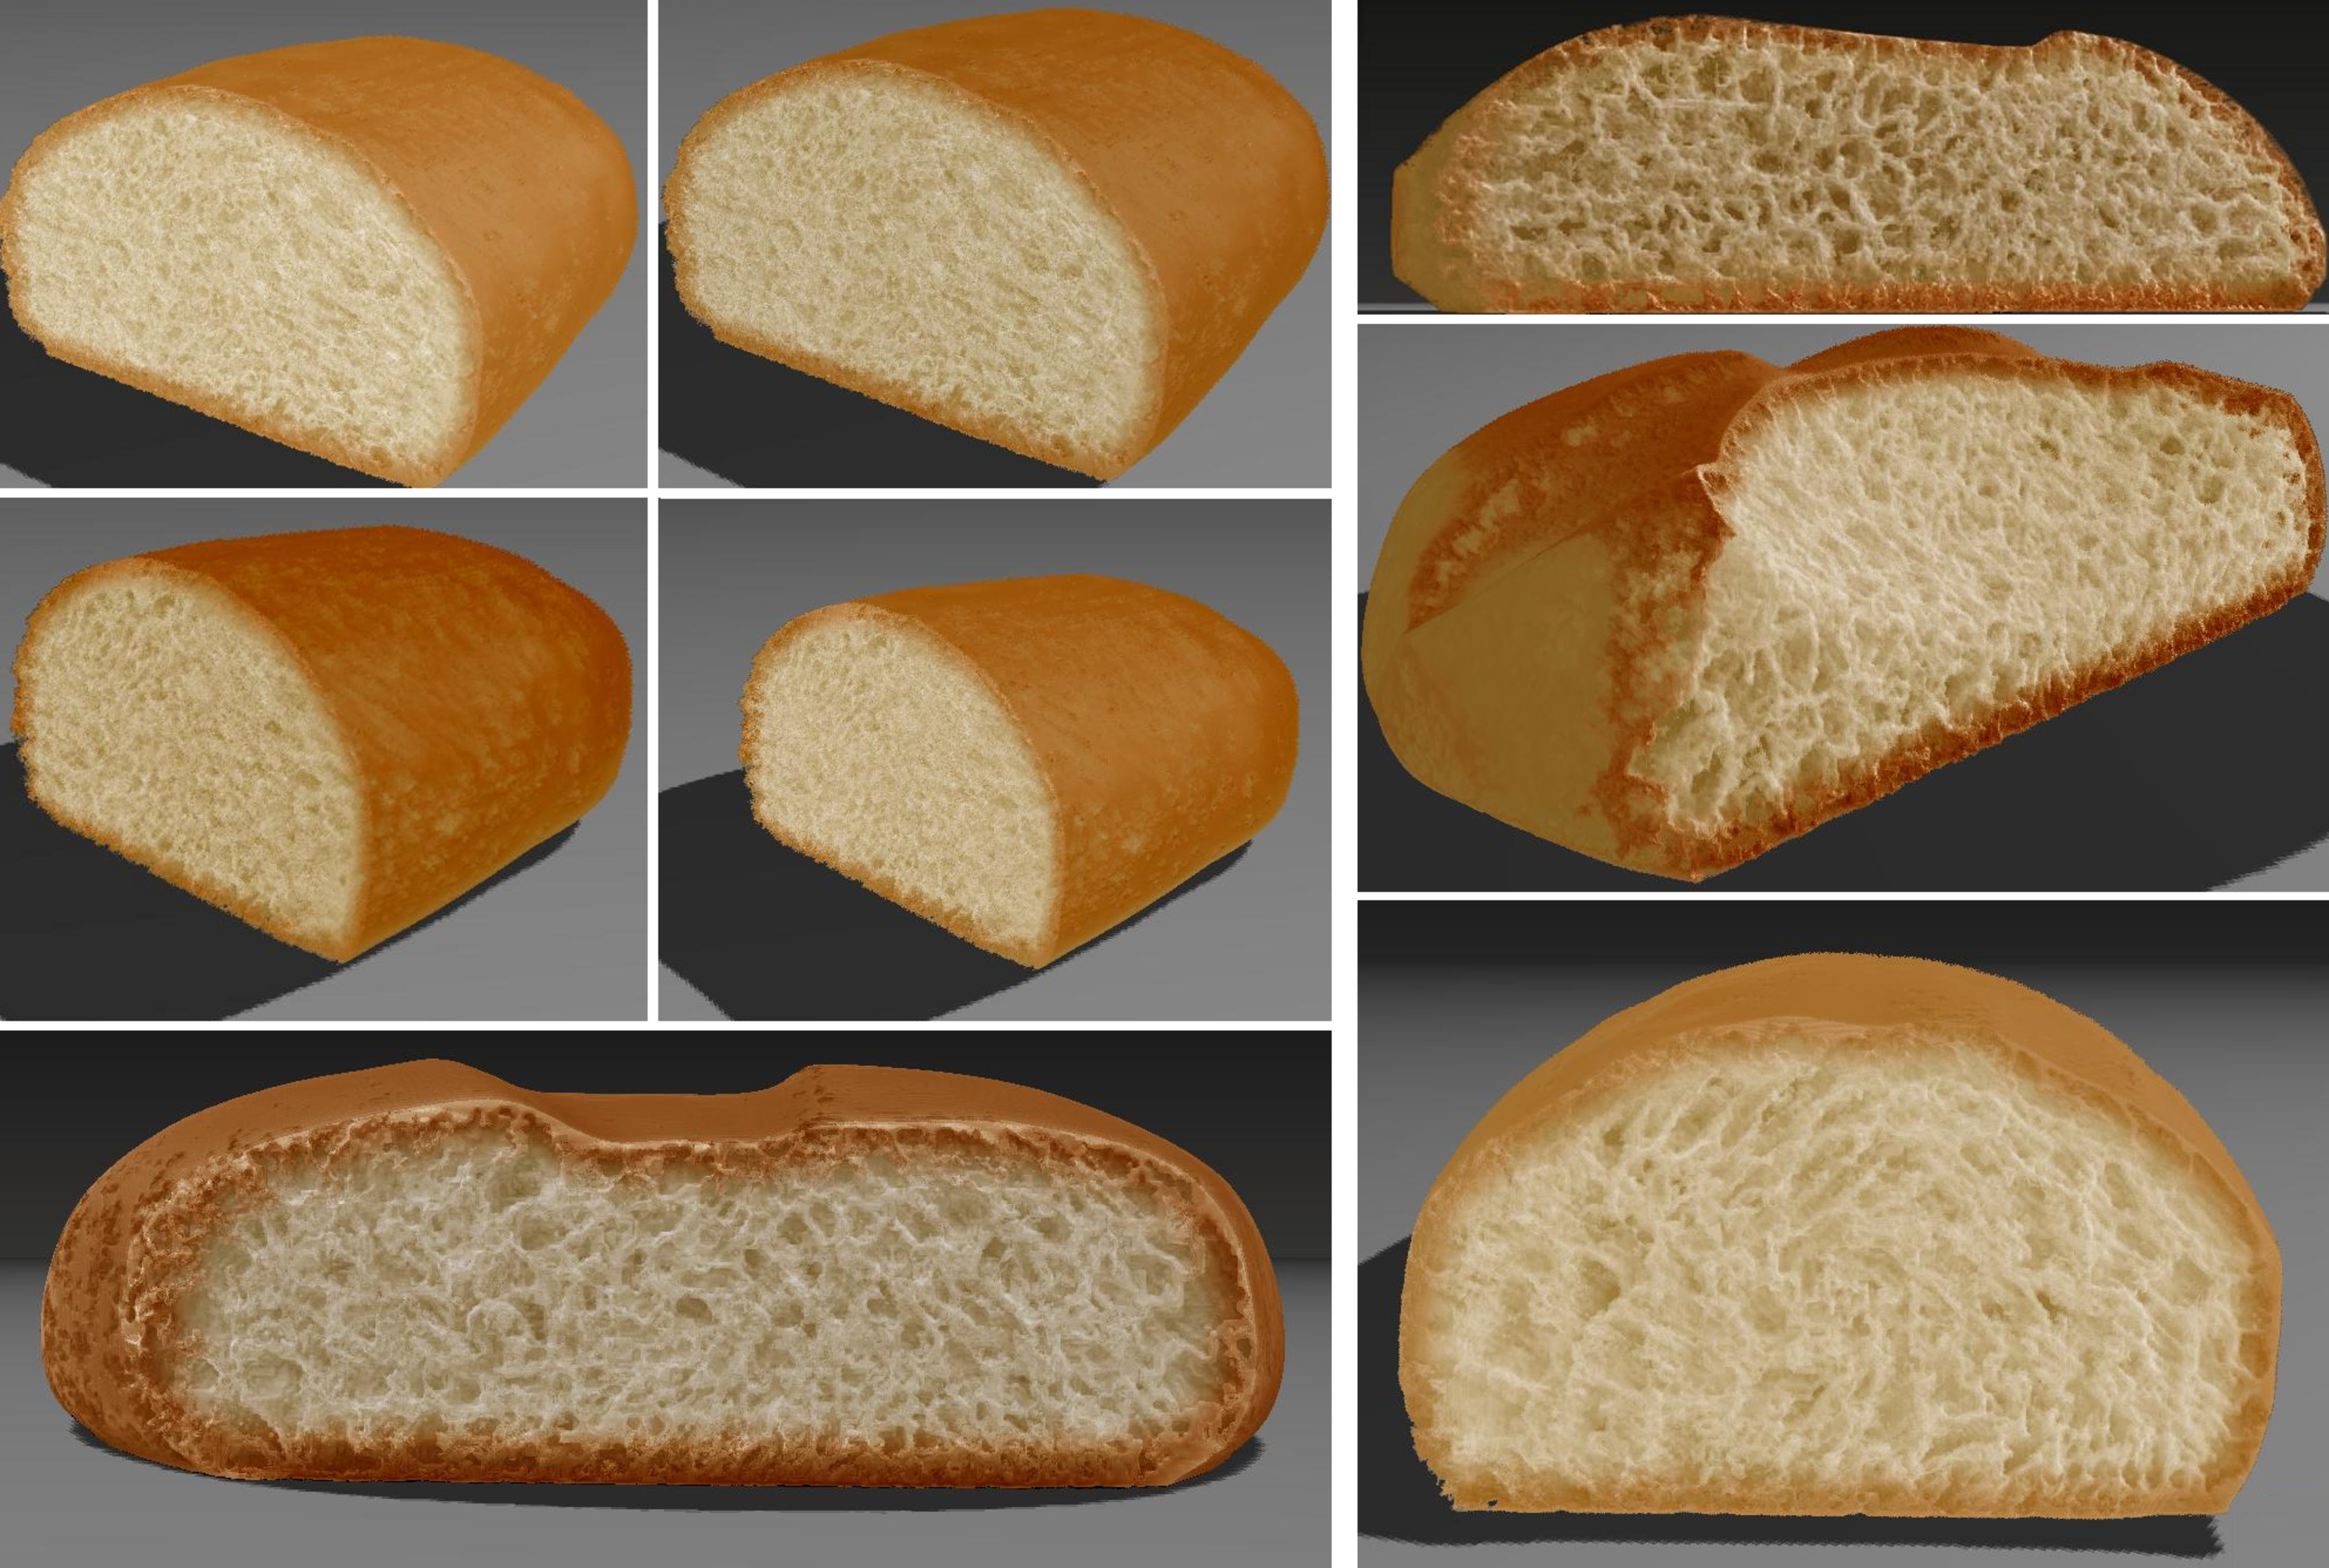
\includegraphics[width=15cm]{figures/Fig12CAVW}}
  \caption{Panes renderizados, utilizando diferentes geometrías y parámetros de renderizado. La imagen muestra que el método simula diferentes apariencias de panes.}
  \label{fg:Fig12}
\end{figure}

\begin{figure}
  \centerline{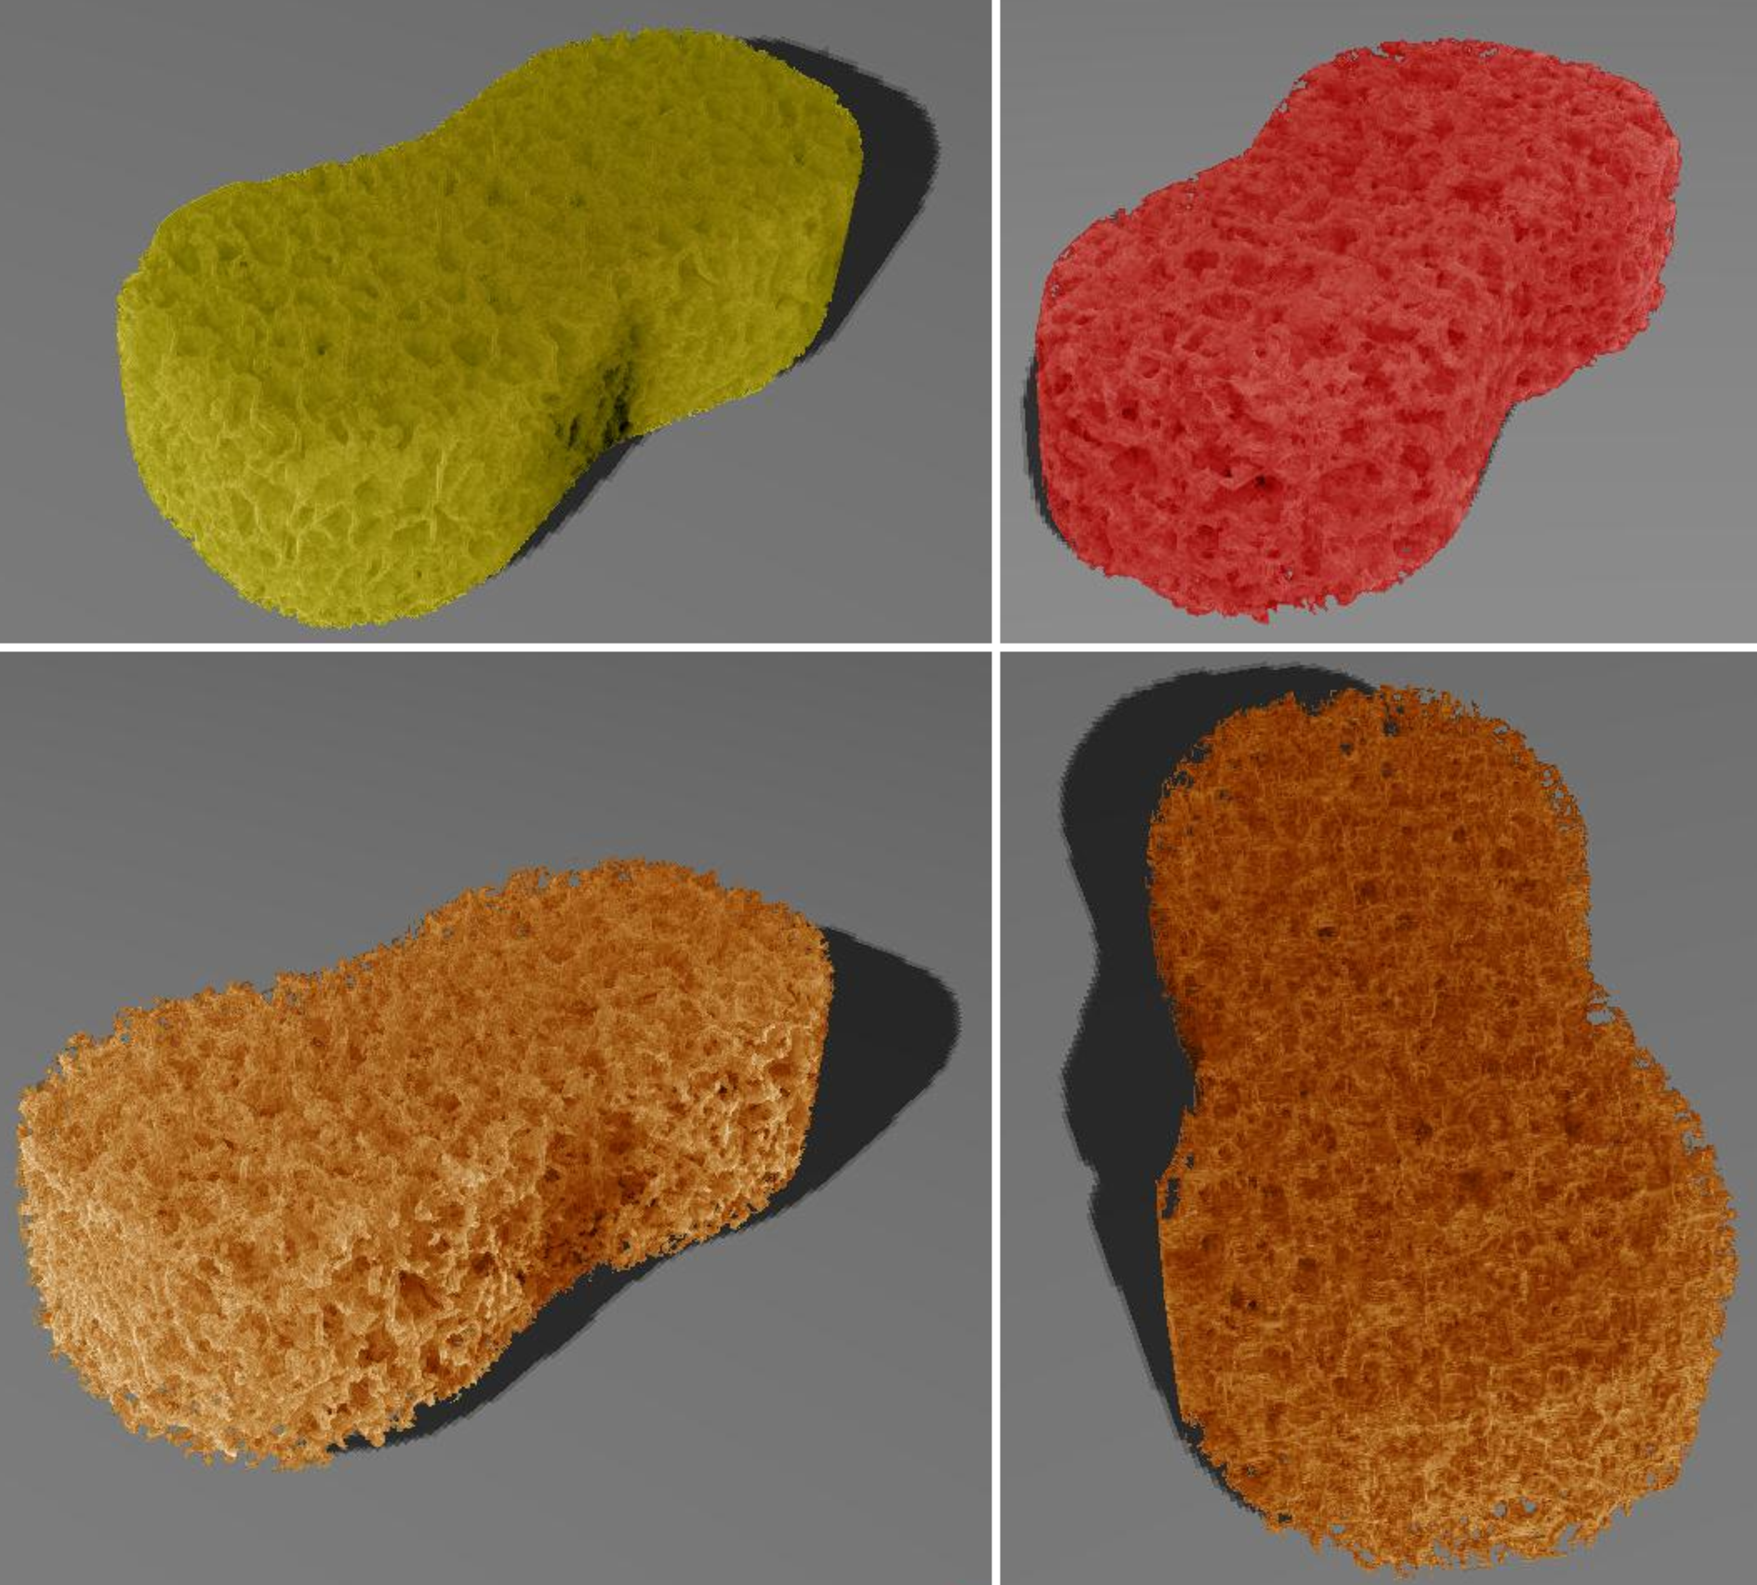
\includegraphics[width=12cm]{figures/Fig13CAVW}}
  \caption{Esponjas renderizadas. La textura volumétrica que representa la geometría fue generada con un valor de {\em aleatoriedad} mayor que en el caso del pan. La geometría resultante posee tamaños y orientaciones de burbujas homogéneos.}
  \label{fg:Fig13}
\end{figure}

\begin{figure}
  \centerline{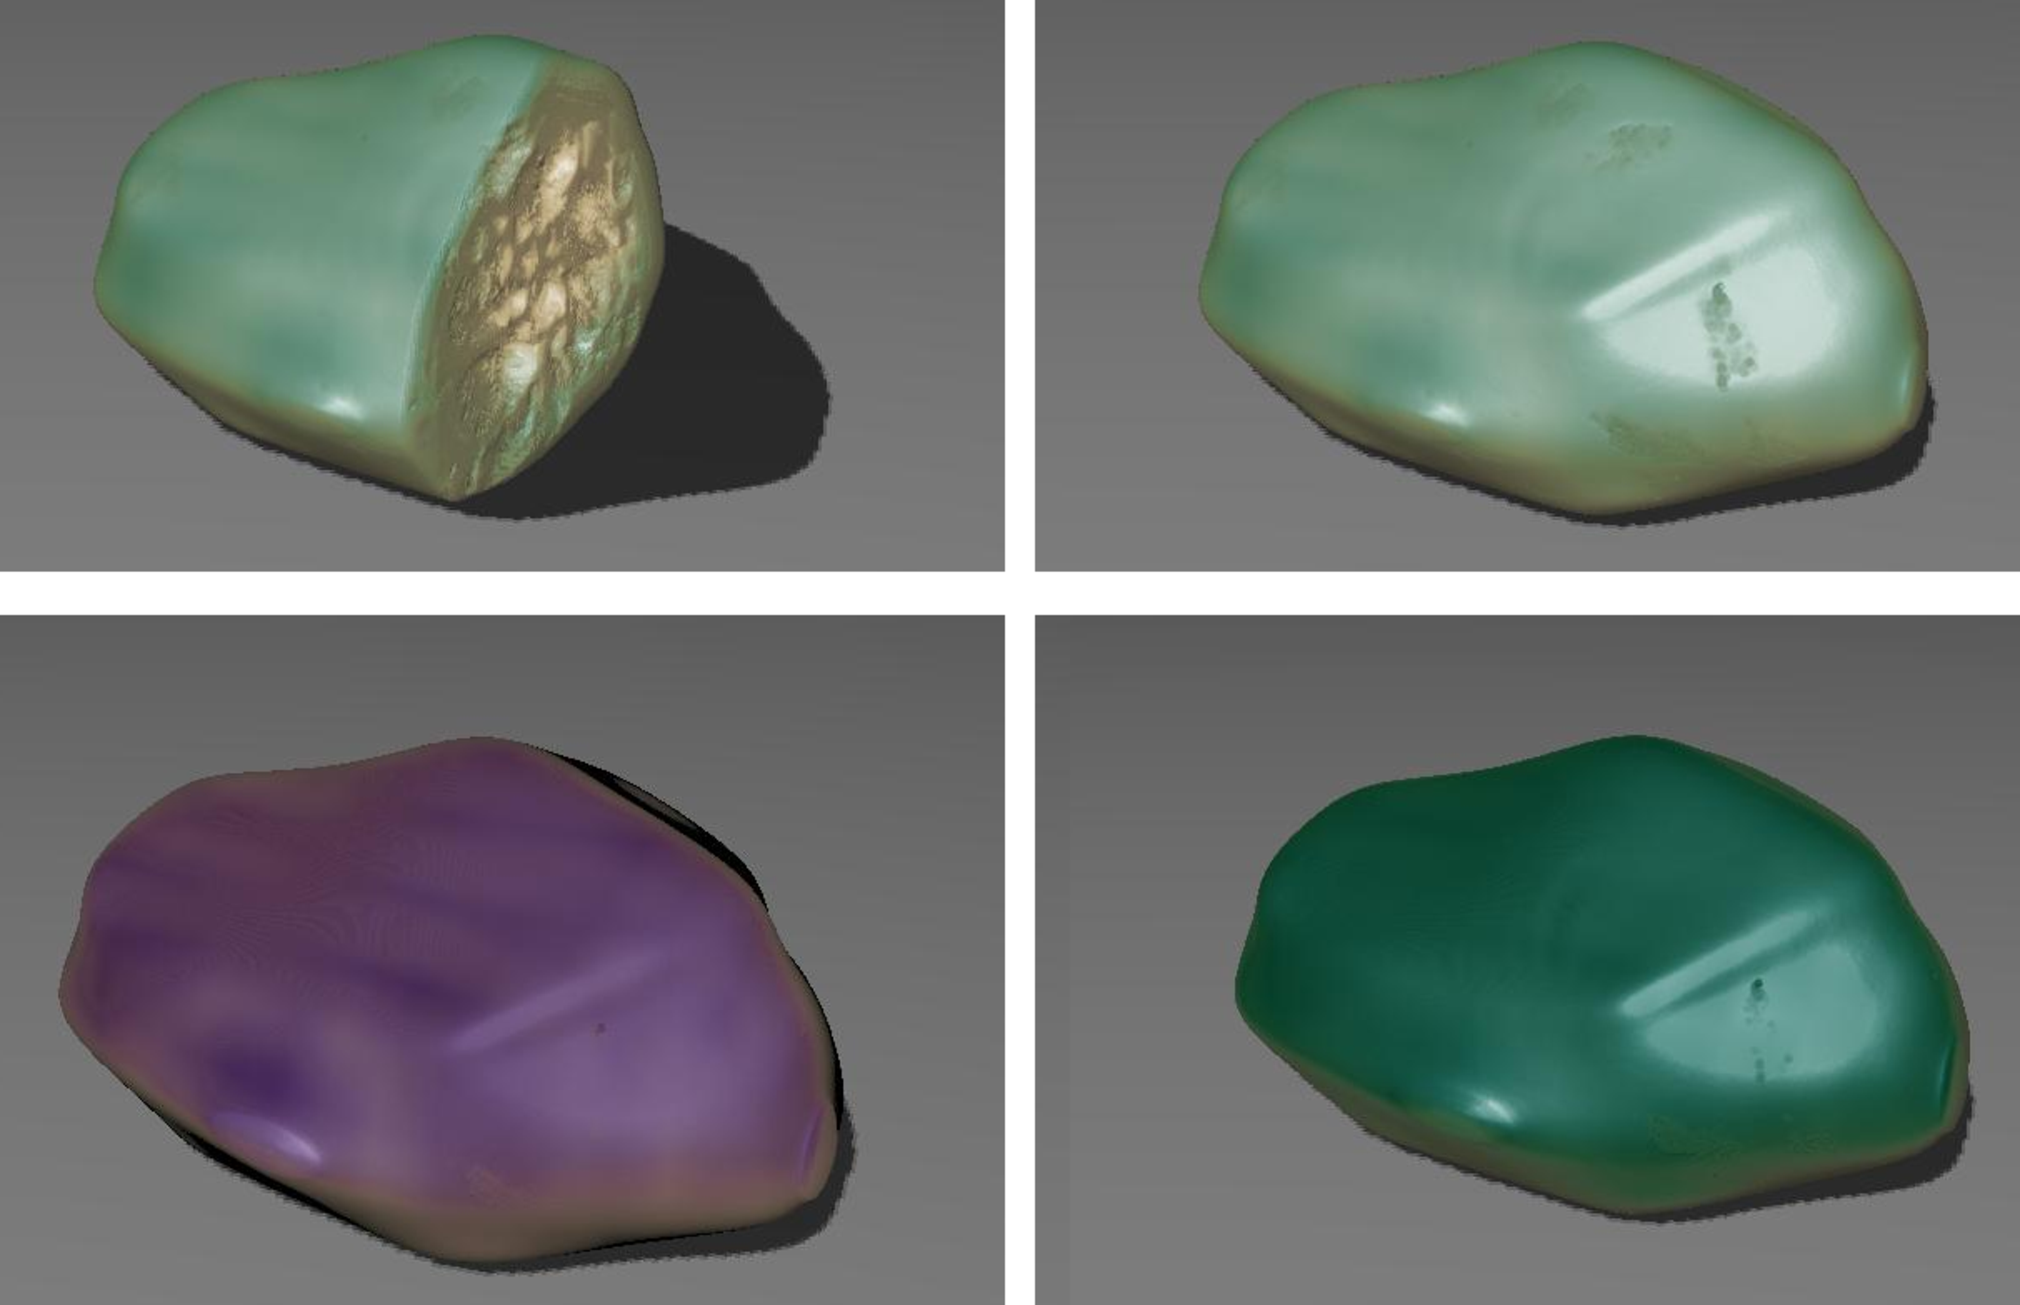
\includegraphics[width=12cm]{figures/Fig14CAVW}}
  \caption{Piedras renderizadas. Se utilizó un menor número de partículas en la generación de este material. El índice de absorción fue incrementado en el renderizado para prevenir una difusión lumínica excesiva.}
  \label{fg:Fig14}
\end{figure}

Debido a estas consideraciones, en la siguiente sección presentamos un algoritmo que demuestra que la elección de un sistema de ecuaciones específico en el diseño permite superar estas deficiencias para el material siendo estudiado.
El mismo continúa la idea de una modelización volumétrica del material, pero está basado en modelos físicos del proceso de fabricación del pan, extraído directamente de la literatura de ingeniería de los alimentos.

\section{Modelado de Pan desde su Proceso de Fabricación}
La obtención de geometrías realistas de la miga de pan requiere comprender su proceso físico de formación.
Utilizando las ideas de la sección anterior, proponemos otro modelo volumétrico de generación de geometrías de migas de pan.
En esta sección proponemos unificar, y diferenciar, los pasos claves presentes en el proceso de fabricación del pan (sobre todo, leudado y cocción).
El procedimiento busca utilizar el proceso físico de generación de geometrías de migas y cortezas de pan a partir de la masa original.
Estos procesos han sido vagamente tenidos en cuenta en la literatura, la cual ha atendido siempre a procesos artísticos más simples, dada la complejidad de los mismos.


\begin{figure*}
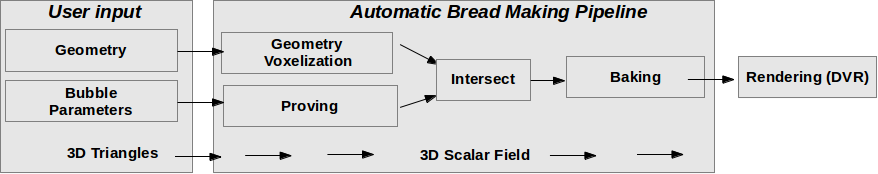
\includegraphics[width=13cm]{figures/pipeline}
\caption{Procedimiento semi-automático para obtener pan sintético foto-realista}
\label{FigPipeline}
\end{figure*}


En primer lugar, reveeremos el estado del arte del proceso de fabricación del pan.
Luego presentaremos los procesos de modelado, que junto con el modelo de iluminación del siguiente capítulo, permiten obtener imágenes foto realistas de distintos tipos de pan.

\subsection{Literatura sobre el proceso de formación del pan}
Si bien existen algunos ejemplos en la literatura sobre modelado y renderizado de la estructura de migas de pan \cite{Tong2005,Xenakis2007}, los mismos ignoran casi por completo el proceso real de formación.
Algunos trabajos pioneros aplicaron modelos físicos de cocción a determinados tipos de pan para su renderizado, buscando obtener animaciones (por ejemplo \cite{Rodriguez-Arenas2011}), pero el modelado de la geometría de las burbujas de la miga del pan no fue tenido en cuenta.

Por otro lado, el modelado procedimental de panes resulta un tópico multidisciplinario de investigación.
La ingeniería de los alimentos lleva varias décadas de publicaciones en el área, tratando de desarrollar una mayor comprensión del proceso de formación del pan.
Esta rama de la ciencia muestra que el leudado determina fuertemente las características presentes en la miga de pan, particularmente las burbujas \cite{Babin2006}.
La interacción entre la levadura y algunos nutrientes presentes en la masa produce {\em $CO_{2}$}. 
El diámetro de las burbujas (asumiendo una burbuja esférica) y sus distribuciones espaciales muestran estructuras con características fractales, exhibiendo autosimilaridad estadística en diferentes escalas de medición.
Determinados trabajos han computado las dimensiones fractales de estas estructuras en determinados tipos de pan \cite{Gonzales2008}, sugiriendo distribuciones fractales uniformes.
El modelado de la cocción del pan es sujeto de numerosos trabajos \cite{Mondal2008}.

El modelado procedimental utilizando fractales también atendió las necesidades de otros variados materiales como montañas \cite{Prusinkiewicz1993}, cráteres lunares, y distribución de las burbujas en quesos \cite{Mandelbrot1983}. 
Adicionalmente, determinados modelos matemáticos complejos representan el comportamiento y el crecimiento de diversos fenómenos naturales.
En computación gráfica, estos modelos son unas de las fundaciones usadas para modelar agua y fluidos \cite{Stam1999,Fedkiw2001}.
Estos trabajos utilizan complejos modelos diferenciales de otras ramas de la ciencia y las aproximan con técnicas numéricas.
En años recientes, la tecnología GPGPU \cite{Owens2007} permitió la posibilidad de alcanzar tiempos reales o interactivos en el cómputo y renderizado de estos modelos numéricos.

A pesar de todos estos avances, el modelado y visualización foto-realista de panes y materiales porosos todavía presenta diversos retos.
Además de un modelo geométrico realista, el renderizado requiere que se represente de manera adecuada los fenómenos de transporte de la luz, incluyendo auto-oclusión, auto-sombreado, transmitancia, translucencia, transparencia, entre otras.
Solamente unas pocas publicaciones proponen atacar ambos aspectos, pero utilizando consideraciones artísticas \cite{Xenakis2007}.
Además, estos autores no liberaron suficientes detalles del modelado y renderización ya que existen derechos de propiedad intelectual, limitando enormemente la reproducción de dichas imágenes.

Por otro lado, la comunidad artística usualmente produce imágenes realistas de pan utilizando fotografías de los mismos, y definiendo geometrías a partir de ellas, junto a la utilización de materiales translúcidos\footnote{http://www.blenderguru.com/tutorials/how-to-create-realistic-bread} y otras consideraciones {\em ad-hoc}\footnote{http://design.tutsplus.com/tutorials/create-a-realistic-loaf-of-bread-in-photoshop--psd-10555}.
Si bien los resultados obtenidos son buenos, los procesos son tediosos y demandan horas de trabajo.
Además, la obtención de una nueva imagen requiere repetir todo el proceso desde el principio, lo que torna al mismo muy poco práctico.
Existen numerosas desventajas además de esta.
Por ejemplo, no se contempla la obtención de cortes arbitrarios del material resultante.


\subsection{Algoritmo de generación procedimental de pan}
La Fig.~\ref{FigPipeline} muestra el proceso completo de formación de geometrías sintéticas de pan.
Todos los pasos se aplican sobre texturas volumétricas.
Los usuarios pueden proveer al sistema con un modelo de tres dimensiones de su preferencia, o dejar que el sistema provea un pan de forma estándar ({\em croissants}, {\em baguettes}, etc.).

La geometría introducida se voxeliza para proceder a las siguientes etapas.
En la simulación del proceso de leudado, el usuario puede parametrizar la textura del pan (cantidad y tamaño de las burbujas y su distribución), o nuevamente dejar que el sistema provea parámetros estándar que producen tipos de pan conocidos.
La masa cruda será intersectada con la geometría voxelizada, obteniendo una textura volumétrica, la cual tiene la forma externa que provee el usuario (o el sistema), con el interior de la misma compuesta de las burbujas procedentes de los parámetros establecidos (ver Sección~\ref{breadprov}).
Luego, se computa un modelo de cocción específico \cite{Powathil2004} el cual deforma la textura volumétrica (y las burbujas de ésta), de acuerdo a los efectos que produce la cocción en el proceso de formación del pan, y a su vez, provoca el levantamiento del mismo, basado en la distribución de burbujas, como ocurre en el proceso real de cocción de este material.
El último paso aplica renderizado directo de volúmenes (direct volume rendering, DVR) \cite{Kruger2003} a la textura volumétrica resultado de la cocción, obteniendo imágenes realistas del pan resultante.

%====================================================================

\subsection{Voxelización de la Geometría}

El modelo permite generar panes con geometrías arbitrarias, supliendo un modelo de triángulos en algún formato estándar.
El modelo consta de una serie de pasos. 
El primer paso de la secuencia voxeliza un modelo provisto por el usuario con la utilidad de código abierto {\tt binvox} \footnote{http://www.cs.princeton.edu/$\sim$min/binvox/} \cite{Nooruddin2003}.
La voxelización genera una textura volumétrica binaria, con $1$ representando que el voxel dado está dentro de la geometría, y $0$ significando que el voxel está fuera de la geometría.
El paso de leudado (siguiente subsección) genera la textura del material que se ubica dentro de esta geometría voxelizada.
Esto permite generar panes con formas arbitrarias, tales como {\em baguettes}, {\em croissants}, pan {\em lactal}, u otros menos comunes (una tetera o un conejo).

Un sub-producto importante de la matriz que representa la geometría está dado por una textura volumétrica secundaria, resultante de una transformación de distancia.
La transformación de distancia genera una matriz $n$-dimensional con las mismas dimensiones que la matriz que se transforma \cite{osh03}.
La transformación computa, para cada entrada en la matriz, la distancia más cercana a una entrada nula de dicha matriz.
Dada una textura volumétrica $M$, el algoritmo genera una textura volumétrica a valores reales $DF_{M}$ con las mismas dimensiones que $M$,


$$DF_{M}[i,j,k] = \min \bigg\{ \delta([i,j,k],[i',j',k']): M[i',j',k'] = 0 \bigg\},$$


\noindent donde $[i,j,k]$ y $[i',j',k']$ son celdas en las respectivas texturas, representando las posiciones espaciales $(i,j,k)$ y $(i',j',k')$, y $\delta$ es la función que computa la distancia entre dos celdas, las cuales pueden ser la distancia de Manhattan, o la distancia Euclideana.
Las entradas de la textura volumétrica lejanas a los bordes del objeto toman valores mayores que aquellas cercanas a los mismos.
De esta manera se obtiene un mapa de la distancia de cada voxel a las superficies tridimensionales del objeto.
Esta textura volumétrica de distancias será requerida en etapas posteriores del proceso.
La Fig.\ref{fg:distance} muestra un ejemplo de un mapa de distancias.

\begin{figure*}
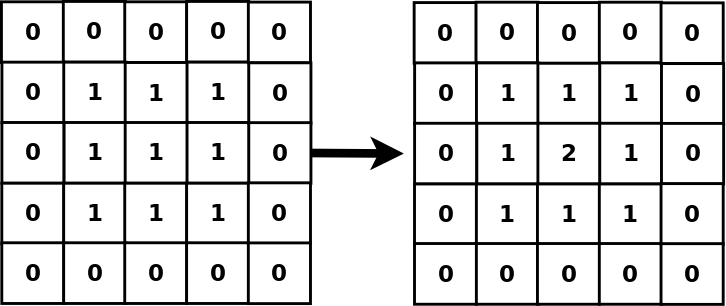
\includegraphics[width=13cm]{figures/distance}
\caption[Mapa de distancias de una matriz bidimensional]{Mapa de distancias de una matriz bidimensional. A la izquierda se observa la matriz original, y a la derecha su mapa de distancias. Se observa que en los bordes el valor del mapa resulta mínimo, aumentando hacia el centro.}
\label{fg:distance}
\end{figure*}


\subsection{Simulación del Leudado}
\label{breadprov}
Como fue discutido, la textura observable en la masa cruda del pan está compuesta de burbujas, cuya distribución exacta resulta de procesos complejos, entre ellos, reacciones químicas, y deformaciones físicas de la masa.
El paso de leudado consta en primera instancia del crecimiento libre de las burbujas, producido por la interacción de seres vivos (levadura) con la masa, la cual libera $CO_{2}$, resultando éste atrapado dentro de la masa.
Luego, el cocinero interviene la masa deformándola de diversas maneras.
En este paso, la masa se deja reposar, efectuándose un segundo leudado.
Finalmente el paso de cocción produce la textura y distribución de burbujas finales.

Debido a la extrema complejidad de los pasos involucrados, las distribuciones exactas de burbujas carecen aún de explicación, por lo tanto existen estudios fenomenológicos sobre estas texturas, las cuales utilizan tomografía de rayos X y extracción de características sobre las mismas \cite{Babin2006,Gonzales2008,VanDyck2014}.
Buscando obtener una variabilidad similar, en esta tesis generamos distribuciones de burbujas con un modelo basado en fractales, inspirado en las distribuciones de burbujas presentes en el queso, y la textura inducida por los cráteres lunares, propuesto en \cite{Mandelbrot1983}.
Luego validamos los mismos utilizando el método multifractal denominado {\em Sandbox} (caja de arena, ya que realiza cálculos sobre una distribución de puntos que asemeja a arena dispersa de manera aleatoria en la geometría).
Esto será explicado en profundidad en el siguiente capítulo (validación).

La textura de la masa se genera procedimentalmente en una textura volumétrica separada, definida en una matriz de tres dimensiones.
Las dimensiones son las mismas de la matriz de geometría definida en la subsección anterior, donde cada voxel se inicializa a $1$ (significando que el material aún no tiene burbujas).
El proceso comienza sustrayendo esferas de radio $r_{min}$ posicionadas arbitrariamente en la textura volumétrica (esto se logra seteando a $0$ las celdas respectivas).
Luego, substraemos esferas de radio mayor, nuevamente en posiciones arbitrarias, hasta un radio máximo $r_{max}$.
La relación entre el número de esferas $N_{s}$ a ser sustraídas en cada paso, y sus respectivos radios $r$, está dada por la ley fractal


\begin{equation*}
N(r) = \frac{k}{r^{d}},
\end{equation*}

\noindent donde $d$ constituye el exponente fractal que modela la ocurrencia de esferas en relación con su radio, y $k$ controla la cantidad de esferas para cada radio.
Con estos simples parámetros basta para modelar una gran cantidad de texturas en general y pan en particular.

La Fig.~\ref{FigProving} muestra un ejemplo de un corte en dos dimensiones de este modelo.
Si bien las burbujas esféricas resultantes no son completamente realísticas debido a su forma, los resultados muestran un notorio parecido en tamaños y distribución de tamaños con binarizaciones de cortes reales de masas leudadas (ver \cite{Babin2006}).
Durante la cocción, la textura volumétrica resultante será sometida a deformaciones geométricas. Consecuentemente, la textura final se ajustará aún más a burbujas de panes reales.
Finalmente, en la sección de validación se buscarán parámetros de generación que ajusten diferentes panes reales. 

\begin{figure}
\center
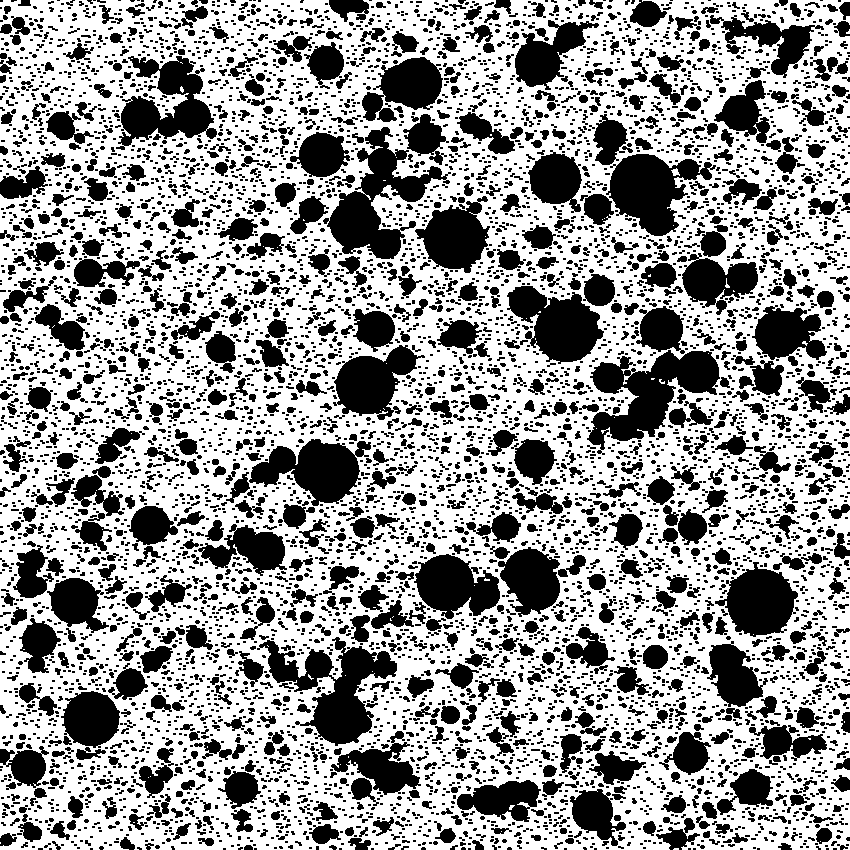
\includegraphics[width=7cm]{figures/bubbles}
\caption{Simulación Fractal del Leudado de Pan.}
\label{FigProving}
\end{figure}

Luego de la voxelización y la simulación de leudado, las burbujas deben estar presentes sólo en el interior de la geometría.
Para esto, intersectamos ambos campos escalares utilizando un simple producto punto a punto, es decir, una máscara, $P_{1} = P \times M$, donde $P_{1}$ nota el campo $3D$ (matriz) que contiene las burbujas del leudado, y $M$ la textura volumétrica que representa a la geometría voxelizada.

La Fig.~\ref{fg:intersectProblem} muestra una versión renderizada de esta intersección.
Si bien los resultados pueden parecer realistas, en panes reales no resulta habitual la visualización de burbujas en la superficie, debido al leudado y cocción reales.
Para solucionar este inconveniente, utilizamos la textura volumétrica de distancias que computamos previamente, para deshabilitar la generación de burbujas en zonas cercanas a los bordes de la geometría, de acuerdo a cierto valor umbral, el cual será un parámetro.


\begin{figure*}
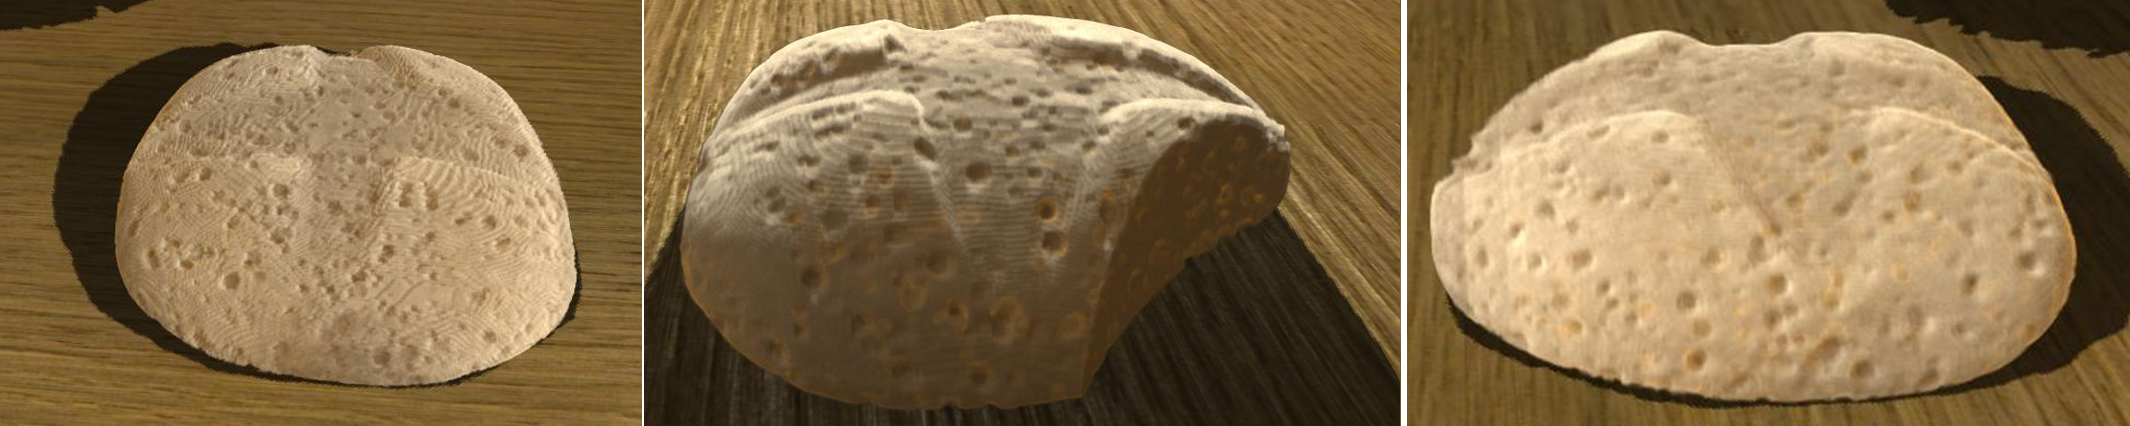
\includegraphics[width=13cm]{figures/intersectProblem}
\caption[Intersección simple de la geometría y de las burbujas provenientes del leudado]{Intersección simple de la geometría y de las burbujas provenientes del leudado. A diferencia de masas reales, pueden verse burbujas en la superficie de la masa.}
\label{fg:intersectProblem}
\end{figure*}


Las Figs.~\ref{fg:proving} y \ref{fg:provingBunny} muestran resultados de limitar las interacciones de burbujas a la región interior de la geometría original, donde se observa que no existen burbujas en la superficie de la masa, como ocurre en masas reales.
Las imágenes muestran que el método definido permite la producción de imágenes realistas de panes crudos con formas arbitrarias.
Cabe remarcar que el modelo resulta suficientemente flexible, permitiendo renderizar el material en cualquier etapa de su proceso de fabricación, además de permitir la posibilidad de realizar cortes arbitrarios sobre el mismo.

\begin{figure*}
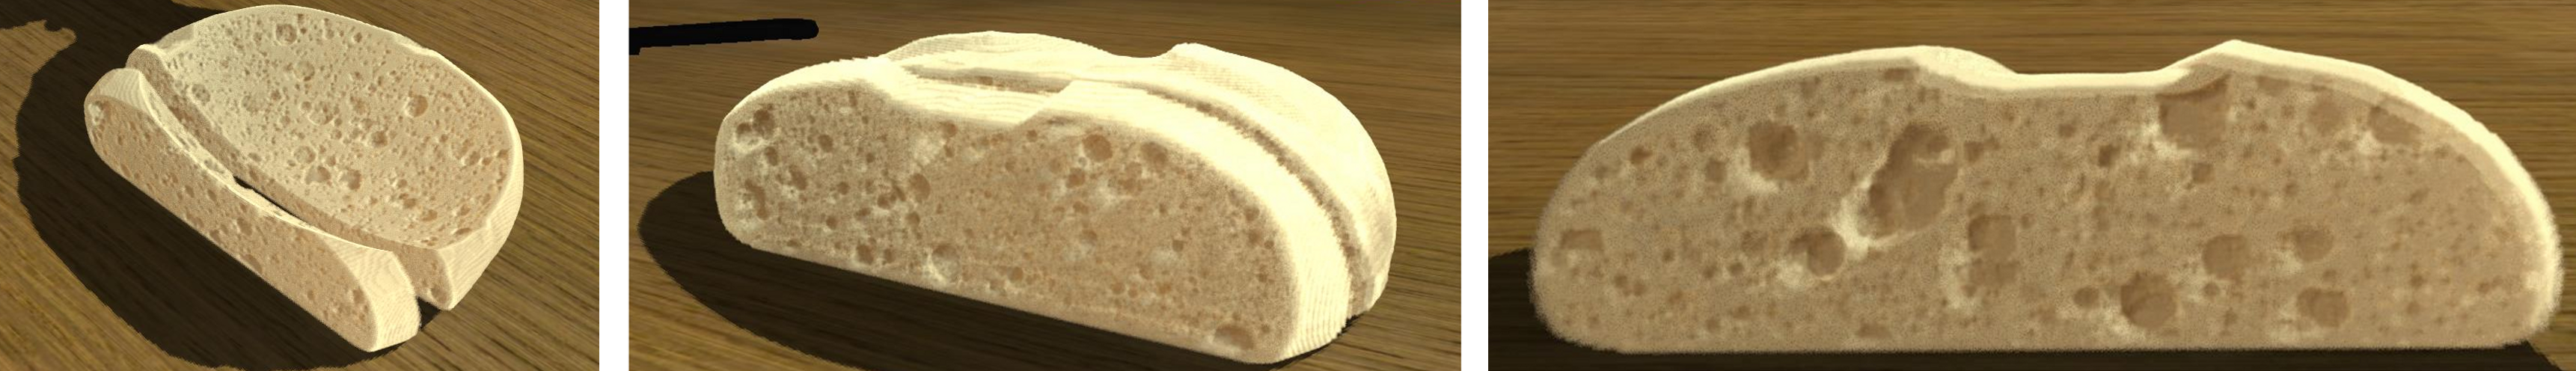
\includegraphics[width=13cm]{figures/prebakebread}
\caption{Pan sintético luego del leudado, y antes de la cocción.}
\label{fg:proving}
\end{figure*}

\begin{figure*}
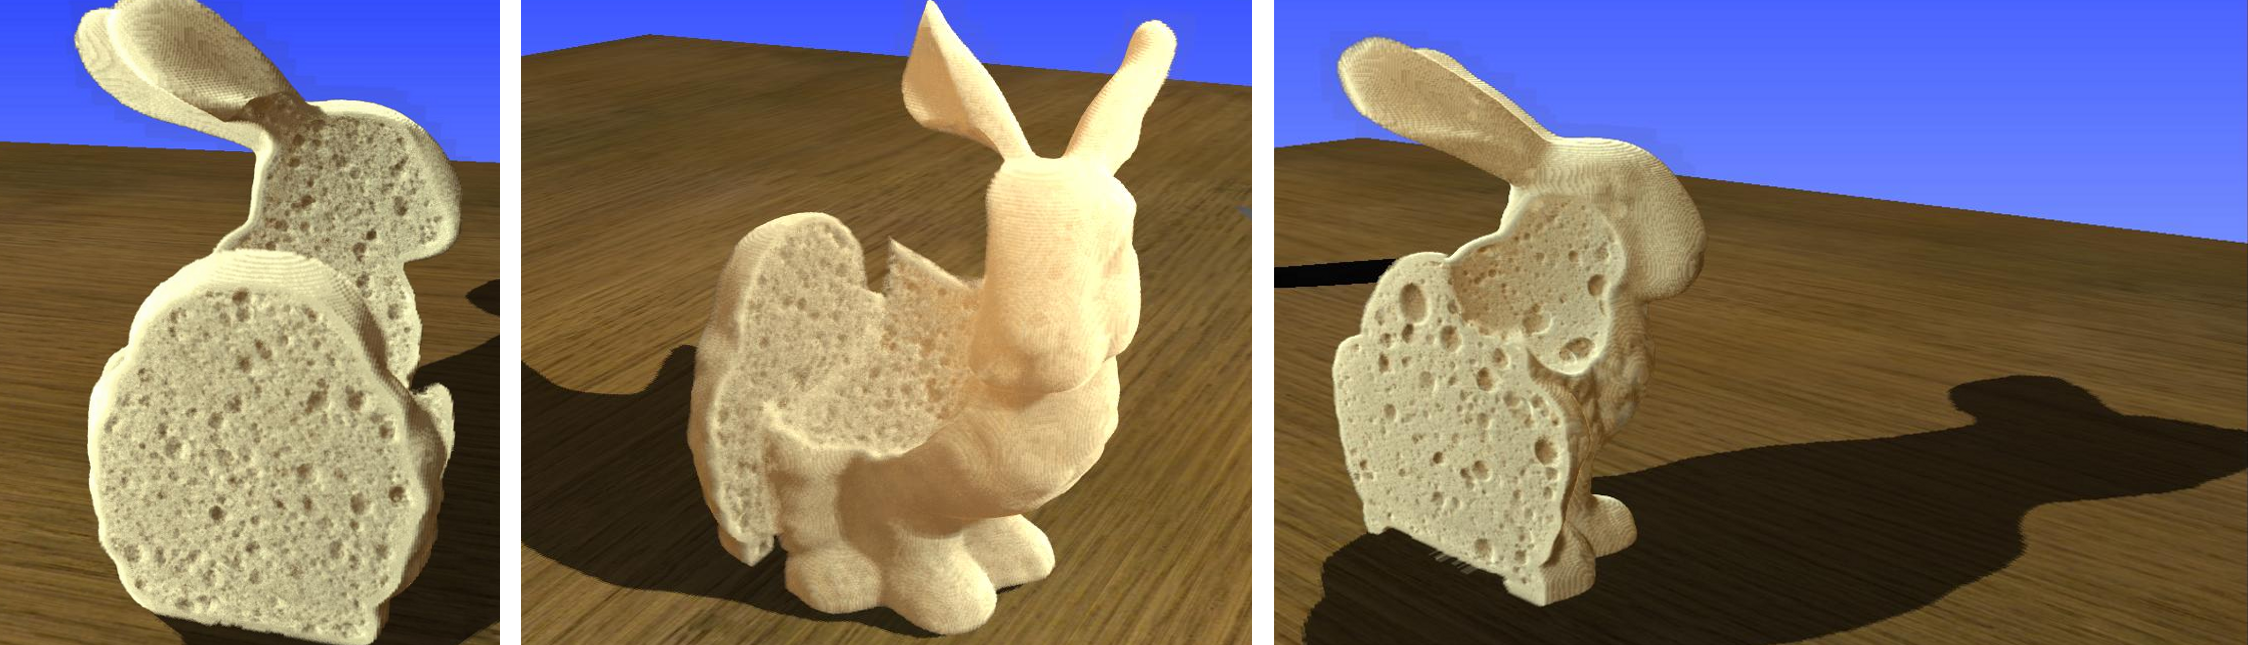
\includegraphics[width=13cm]{figures/prebakebunny}
\caption{Conejo de pan sintético, luego del leudado, y antes de la cocción.}
\label{fg:provingBunny}
\end{figure*}

%====================================================================
\subsection{Cocción}
Los modelos matemáticos del proceso de cocción del pan deben ser capaces de modelar correctamente las transferencias de calor y masa en el mismo.
Los modelos físicos más completos del proceso producen soluciones precisas a la distribución de temperaturas en la masa durante la cocción.
Sin embargo, estos modelos poseen una implementación muy compleja, y resultan muy costosos computacionalmente.
Además, sólo los modelos más complejos toman en consideración la formación de la corteza del pan.
La corteza, por otro lado, aún carece de una definición formal~\cite{Vanin2009}.
Por lo tanto, los modelos antes citados incluyen sólo una simplificación de la formación de la misma, muy lejos de lo que ocurre en la cocción real.

\subsubsection{Deformación de las burbujas utilizando la temperatura}
Los resultados más relevantes en la literatura sugieren que un modelo unidimensional de la cocción puede ser suficiente para la mayoría de los casos prácticos.
Por ejemplo, Purlis~\cite{Purlis2011} modela la cocción del pan como un fenómeno unidimensional, representando la geometría como un cilindro infinito.
Otros trabajos asumen sólo una coordenada radial, resultando también en modelos $1D$~\cite{Powathil2004, Thorvaldsson1999}.
Estos trabajos muestran que utilizar una representación de una única dimensión produce resultados casi idénticos a aquellos que se obtienen utilizando un mayor número de dimensiones.

La simulación numérica que implementamos está basada en el esquema de diferencias finitas propuesto por Powathil~\cite{Powathil2004}, y Thorvaldsson y Janestead~\cite{Thorvaldsson1999}. 
El sistema presentado consiste de un conjunto de tres ecuaciones acopladas que describen transferencia de calor, difusión de vapor de agua y difusión de agua líquida.
En nuestro algoritmo, sólo utilizamos las temperaturas ($T$) como entrada para las siguientes etapas de la formación del pan.
La Ec.~\ref{Eq:heat} modela transferencia de calor en la masa del pan, tomando en consideración el balance de energía y evaporación del agua debido a la temperatura~\cite{Thorvaldsson1999},
%
\begin{equation}
\label{Eq:heat}
\frac{\partial T}{\partial t} = \frac{1}{\rho C_{p}} \frac{\partial}{\partial x} \left ( k \frac{\partial T}{\partial x} \right ) + \frac{\lambda}{C_{p}} \frac{\partial W}{\partial t}+\frac{\lambda W}{ \rho C_{p} }\frac{\partial \rho}{\partial t},
\end{equation}
%
\noindent donde $T$ representa la temperatura, $x$ es la coordenada radial, $t$ es el tiempo, $C_{p}$ el calor específico, $\rho$ la densidad, $k$ la conductividad térmica, $\lambda$ es el calor latente de la evaporación de agua, y $W(x,t)$ es el contenido de agua líquida. 
Las condiciones iniciales
%
\begin{align*}
T(x,0) &= T_{0}(x), 0\le x \le L/2,
\end{align*}
y las condiciones de borde (continuidad y suavidad) definen el modelo,
\begin{align*}
\left ( \frac{\partial T}{\partial x} \right )_{x=L/2} &= 0 , t > 0 \\
-k \left ( \frac{\partial T}{\partial x} \right )_{x=0} &= h_{r}(T_{r}-T_{s}) + h_{c}(T_{air}-T_{s}) - \lambda \rho D_{w} \left (\frac{\partial W}{\partial x} \right )_{x=0}
\end{align*}
%
\noindent donde $h_{r}$ y $h_{c}$ son sub-términos del coeficiente de transferencia de calor ($h = h_{r}+h_{c}$), $T_{air}$, $T_{s}$, $T_{r}$ son temperaturas en el aire circundante, en la superficie del pan, y en la fuente de radiación, respectivamente, $L$ es el diámetro del pan ($x = L/2$ se ubica en el centro del pan y $x = 0$ en el contorno del mismo), $D_{w}$ representa la difusividad del agua líquida, y $T_{0}$ la temperatura inicial. 
Las temperaturas están expresadas en Kelvin ($K$). 
El modelo consta de ecuaciones similares para la difusión del vapor de agua ($W$) y difusión de agua líquida ($V$).
Otros detalles del modelo pueden ser consultados en \cite{Thorvaldsson1999}.
En nuestro trabajo, utilizamos este modelo para obtener un mapa de temperaturas al final del proceso de cocción.
Estas temperaturas afectarán posteriormente las formas y tamaños de las burbujas.

La simulación de la cocción define el horno a una temperatura típica (por defecto utilizamos $210^{\circ}C$) y discretiza el tiempo en intervalos $\Delta t = 30s$.
De la simulación se obtiene un arreglo unidimensional $Temp$, de tamaño $N_{grid}$, compuesto por valores de temperatura.
Por estabilidad numérica, utilizamos $N_{grid}=32$ (como en el trabajo original) e interpolamos las temperaturas para obtener mayores resoluciones ($N_{int}$). 
%Each value represents a dough position after $M$ baking time steps. 

El vector obtenido presenta temperaturas decrecientes de $R = 0$ a $R = L/2$, ya que el centro y el borde del pan poseen la menor y la mayor temperatura, respectivamente, luego de la cocción (el calor fluye desde la corteza hacia el centro del pan). 
Si utilizamos la textura volumétrica de distancias computado previamente, en conjunto con el vector de temperaturas, podemos mapear distancias a temperaturas.
Esto permite definir temperaturas en la textura volumétrica de forma compatible a una simulación $3D$.
Basados en estos razonamientos, mapeamos el vector de temperaturas $Temp$ en $3D$ de la siguiente manera,
\begin{equation*}
\displaystyle R_{vol}[x,y,z] = Temp[ round( DF_{M}[x,y,z] ) ], 
\end{equation*}
%
\noindent donde $R_{vol}$ es la textura volumétrica resultante del mapeo, y $x$, $y$ y $z$ son coordenadas $3D$ en $R_{vol}$. Cuando $DF_{M}[(x,y,z)] = 0$, la posición actual $3D$ se encuentra en la superficie de la geometría, y $Temp[0]$ se mapea $R[(x,y,z)]$.
Cuando $DF_{M}[(x,y,z)] > 0$, mapeamos una temperatura menor a $R_{vol}$, ya que la posición actual se encuentra en el interior de la geometría.
La Fig.~\ref{fg:baking} muestra cortes del resultado de este mapeo ($R_{vol}$), usando temperaturas resultantes de un tiempo arbitrario de cocción, en los tres planos Cartesianos. 
Las imágenes son casi idénticas a lo que se obtendría con una simulación $3D$~\cite{Purlis2010}.

\begin{figure*}
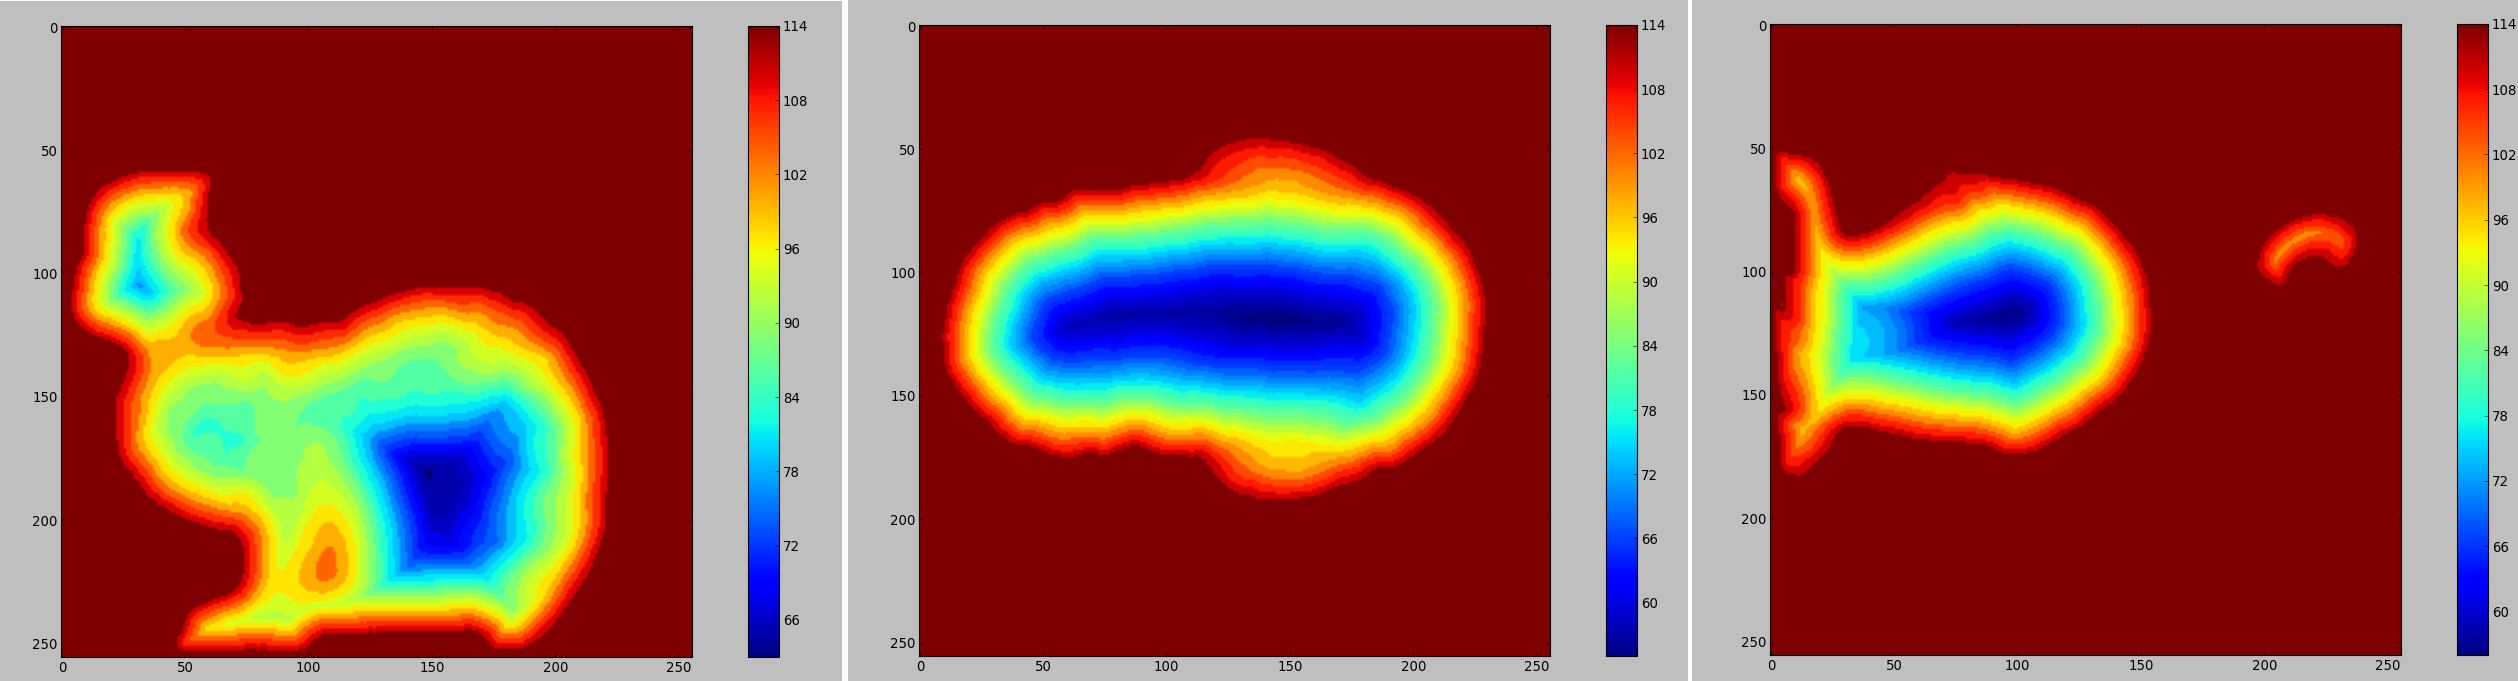
\includegraphics[width=13cm]{figures/tempsbunny}
\caption[Temperaturas unidimensionales mapeadas a una textura volumétrica con forma de conejo]{Temperaturas unidimensionales mapeadas a una textura volumétrica con forma de conejo. Las imágenes muestran que la distribución de temperaturas arroja resultados similares a una simulación en tres dimensiones.}
\label{fg:baking}
\end{figure*}

Luego de cierto número de pasos de simulación ($t=20$ en nuestro caso), computamos el campo vectorial del gradiente de $R_{vol}$ \cite{Gonzalez2006}, $g$, y luego suavizamos el mismo utilizando un kernel Gaussiano, obteniendo $g'$.
Finalmente, utilizamos las versiones suavizadas para deformar la textura volumétrica de la siguiente manera,
\begin{align*}
\displaystyle
[x,y,z] = [u,v,w] + p\, g'[u,v,w],
\end{align*}

\noindent donde $[u,v,w]$ son las coordenadas en la textura volumétrica original, y $[x,y,z]$ son las coordenadas resultantes, $p$ es un parámetro real positivo que denota la intensidad con la que se deforma el campo (controla el efecto neto de la cocción en las burbujas), y $g'$ es las versión suavizadas del gradiente original $g$.
La Fig.~\ref{fg:bakedbubbles} muestra cortes $2D$ de campos escalares luego de aplicado el proceso de deformación por temperatura a diferentes formas.

\begin{figure*}
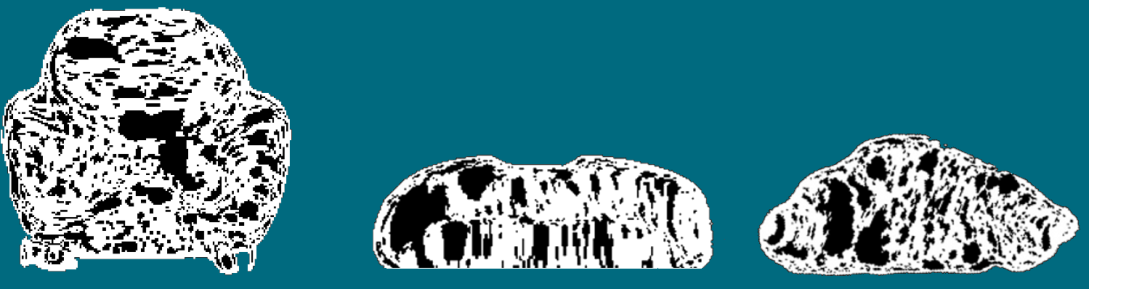
\includegraphics[width=13cm]{figures/bakedbubbles}
\caption{Cortes bidimensionales con burbujas deformadas por el proceso de deformación en diferentes tipos de panes.}
\label{fg:bakedbubbles}
\end{figure*}

El parámetro $p$ puede ser utilizado para sintetizar diferentes apariencias de miga de pan, desde masa cruda hasta burbujas con mucha deformación (ver Fig.~\ref{fg:parameterp}).
Cuando incrementamos $p$, forzamos a las burbujas a seguir más ajustadamente la forma exterior del pan. 
La imagen también muestra que el método deforma más pronunciadamente las burbujas más cercanas a la corteza.
Finalmente, en la imagen puede observarse el elongamiento de las burbujas, paralelo a la pared derecha del pan.

\begin{figure*}
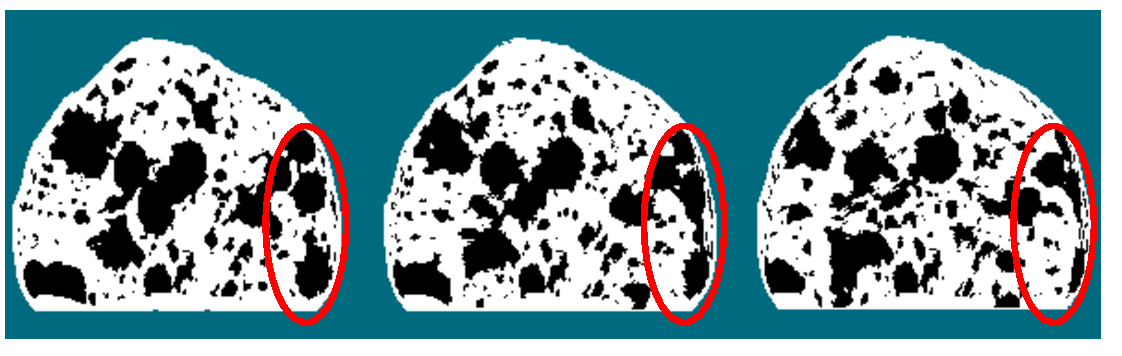
\includegraphics[width=13cm]{figures/parameterp}
\caption[Efecto del parámetro $p$ en la simulación de cocción]{Efecto del parámetro $p$: de izquierda a derecha $p$ es $5$, $10$, y $15$ respectivamente. Las burbujas son presionadas de manera realista hacia la corteza del pan.}
\label{fg:parameterp}
\end{figure*}

\subsubsection{Crecimiento de la Masa}
El crecimiento de la masa constituye uno de los fenómenos más visibles durante el proceso de cocción del pan.
Esto se debe a que las temperaturas producen la liberaación de $CO_2$ en las burbujas atrapadas en la masa, resultando en un crecimiento global del pan.

La literatura muestra que, en escenarios típicos, la masa del pan crece hasta el doble en volumen \cite{Fan1999}, dependiendo de las condiciones del horno.
En nuestro modelo, este proceso puede ser simulado utilizando la distribución de burbujas y sus radios, provenientes del proceso de leudado.
Esta información la computamos creando una textura volumétrica auxiliar $P$, donde en cada entrada se computa el radio de las burbujas que ocurren en esa entrada, de la siguiente manera:

$$P[x,y,z] = max \bigg\{r\bigg\},$$

\noindent donde $r$ es el radio de una burbuja que ocurre en la entrada $[x,y,z]$.
El término $max$ en el cómputo retiene el máximo radio que ocurre en la entrada $[x,y,z]$.
Buscando obtener transiciones suaves de radio en la textura final, se aplica un filtro Gaussiano a $P$.
Esta textura volumétrica permite definir distintas funciones útiles que simular aproximaciones plausibles del crecimiento de la masa durante la cocción.

El volumen original será deformado con los valores provenientes de $P$, obteniéndose diferentes crecimientos para diferentes radios.
De esta forma, el valor $p$ de la sección anterior es reemplazado por el valor de $P$ correspondiente a cada posición.
Matemáticamente, se deforma en sistema de coordenadas de la siguiente forma:

\begin{equation*}
[r,s,t] = [u,v,w] + P[u,v,w] \, g'[u,v,w], \\
\end{equation*}

\noindent donde $[u,v,w]$ es la entrada original, y $[r,s,t]$ es la coordenada deformada.

El crecimiento se produce por medio de escalamiento local: deformamos la textura volumétrica auxiliar utilizando una función que la escala, por medio de un parámetro con valor real $S > 1$, y el valor del radio de la burbuja en la entrada correspondiente:

\begin{equation}
\label{Eq:rise}
[x,y,z] = [r,s,t]\, S \, P[r,s,t],
\end{equation}

\noindent donde $[x,y,z]$ es la entrada final, luego de la deformación inducida por el crecimiento.

La Fig.~\ref{fg:rising} muestra ejemplos de masas antes y después del crecimiento.
La imagen muestra también diferentes crecimientos para burbujas de distintos tamaños.
Además se puede observar que, de la misma manera que en los panes reales, se produce el fenómeno de coalescencia (unión) en las burbujas que crecen.
Las diferencias en tamaño pueden ser aleatorizadas para obtener crecimiento variable en las burbujas.

\begin{figure*}
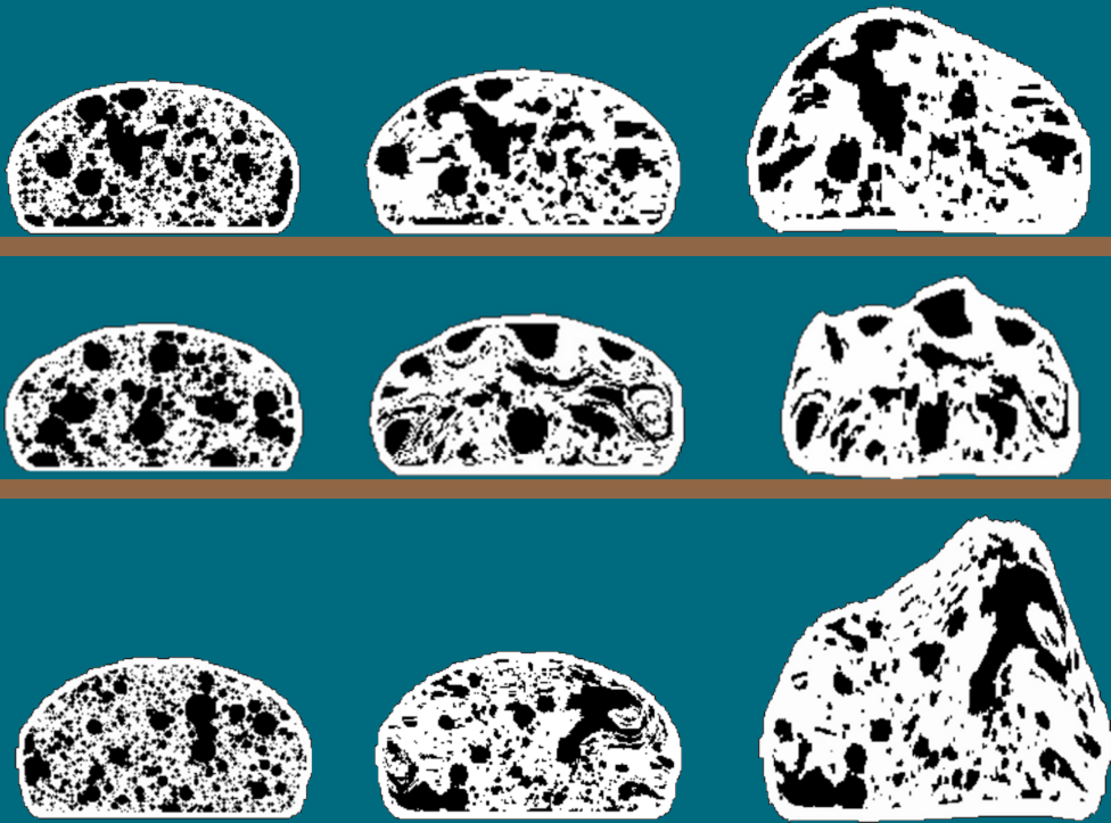
\includegraphics[width=13cm]{figures/Fig9}
\caption{Ejemplos de crecimiento de la masa, utilizando distintos valores de $S$. La imagen muestra el efecto de la cocción en la forma global de la masa y en las burbujas en particular. Diferentes crecimientos y coalescencias se observan en las burbujas. }
\label{fg:rising}
\end{figure*}


\subsection{Formación de la Corteza}
El modelo de cocción introducido no incluye detalles precisos de la formación de la corteza.
En estas ecuaciones, esta se asume como un sub-producto que se produce en la superficie del material, a determinada temperatura, pero esta simplificación constituye sólo una cruda aproximación al fenómeno en el proceso real de cocción.
La literatura de ingeniería de los alimentos define la corteza como una interfase que emerge entre la masa y el aire.
Entre sus principales características se encuentra la formación de un material más denso en la superficie, y una diferenciación de color.
Sin embargo, los detalles precisos acerca de cómo esto ocurre se desconocen, por lo tanto, la apariencia exacta de la misma, está lejos de ser comprendida en los modelos presentes actualmente.

Debido a esto, y basados en la aproximación inicial asumida, utilizamos la textura volumétrica de distancias computada previamente para definir una región de corteza.
Esta elección está fundada en el hecho de que la corteza está mayormente determinada por un frente de evaporación que resulta de la temperatura \cite{Jefferson2007}.
En otras palabras, obtenemos las posiciones de la corteza utilizando la textura volumétrica mencionada, ya que hemos definido una relación entre la temperatura y la distancia a la superficie.
Además, obtenemos diferentes apariencias de pan utilizando un parámetro de distancia que determina diferentes espesores de corteza.

Adicionalmente, utilizamos colores medidos en el proceso real de cocción \cite{Purlis2009}, para determinar diferentes apariencias de la corteza.
Utilizamos el canal $L$ del espacio de color CIELab \cite{Hunter58} para controlar la historia de cocción en cada voxel de la corteza.
Dicho canal determina la {\em luminancia}, mientras uqe los canales restantes, $a$ y $b$, determinan la cromaticidad.
En \cite{Purlis2009} fue determinado que los valores del canal $L$ varían aproximadamente entre $90$ (crudo) y $40$ (quemado).
Los valores de los canales de cromaticidad fueron elegidos utilizando colores medidos en imágenes de panes reales.
Esta información nos permitió definir un rango de colores $CIELab$, los cuales varían suavemente de crudo a completamente cocido. 

Los colores definidos pueden ser distribuidos sobre la superficie de la corteza por medio de consideraciones artísticas.
Por ejemplo, es posible utilizar nuevamente información proveninente del proceso de leudado ({\em e.g.}, el radio de la burbuja más cercana), e incluso ruidos procedimentales ({\em e.g.}, Perlin).
En cada entrada de la corteza, los valores obtenidos de estas funciones se utilizan para elegir un color de los colores definidos.

En nuestro caso, definimos la {\em densidad de la corteza} en cada posición de la textura volumétrica como $N_{v} / W_{size},$ donde $N_{v}$ es el número de voxels con valor $1$ en una ventana en el entorno de la posición, y $W_{size}$ es el número de voxels en esa ventana.
Luego utilizamos este valor para modular el canal $L$ en el color en cada posición, obteniendo imágenes plausibles.
La función fue definida debido a la siguiente observación: en los lugares de la corteza donde hay menos masa (por ejemplo, esquinas), el efecto de la cocción es más marcado.
El tamaño de la ventana puede ser utilizado para obtener variabilidad en la apariencia de la corteza.
%Por completitud presentaremos además otro método, basado en morfología matemática, para calcular la región del volumen que representa la corteza.

%\subsection{Determinación de la corteza utilizando morfología matemática}
%Debido a que resulta difícil o imposible definir funciones matemáticas algebraicas que se adapten a cualquier forma, proponemos un método automático para determinar regiones exteriores de volúmenes utilizando el formalismo conocido como morfología matemática \cite{Gonzalez2001}.

%Con esto se pretende obtener una región que se ajuste a los bordes de una textura volumétrica.
%Para esto se utilizarán técnicas simples conocidas como apertura, cierre, erosión y dilatación.
%Las operaciones las definiremos en campos escalares tridimensionales.

%Un elemento estructurante $E$ denota una textura volumétrica binaria que representa una forma particular (cubo, esfera, etc.).
%Los elementos estructurantes son utilizados en la definición de las operaciones antes mencionadas.

%La operación de erosión se utiliza para reducir el tamaño total de la textura volumétrica.
%La erosión de una textura volumétrica $A$ utilizando un elemento estructurante $B$ se define de la siguiente manera,

%\begin{equation}
%A \ominus B = \{z\in \mathbb{Z}^3 | B_{z} \subseteq A\},
%\end{equation}

%noindent donde $B_{z}$ es la traslación de $B$ por el vector tridimensional $z$.

%La dilatación aumenta el tamaño total de la textura volumétrica, preservando en cierta manera la forma de sus bordes.
%La dilatación de una textura volumétrica $A$ utilizando el elemento estructurante $E$ se define como sigue,

%\begin{equation}
%A  \oplus E = \bigcup_{e\in E} A_e.
%\end{equation}

%La operación de cierre se emplea para {\em cerrar agujeros} en la textura volumétrica.
%El cierre de un campo $B$ utilizando un elemento estructurante $E$ se define como una dilatación seguida de una erosión,

%\begin{equation}
%B \bullet E = (B \oplus E) \ominus E,
%\end{equation}

%\noindent ver \cite{Gonzalez2001} para obtener mayores detalles.

%Para obtener la región externa de la geometría representada en la textura volumétrica, se necesitan eliminar los agujeros internos que representan las burbujas.
%Para esto, el primer paso produce un cierre $c$ de la textura volumétrica utilizando un cubo (elemento estructurante de radio $r$), causando el cierre de las burbujas internas.
%Llamaremos $d$ a la dilatación de $c$ con un elemento esférico de radio $r_{2}$ ($d = c \oplus E_{r_{2}}$) y $e$ a la erosión de $d$ utilizando un elemento estructurante esférico con un radio ligeramente menor ($r_{3}$), $e = d \oplus E_{r_{3}}$.
%La diferencia entre $d$ y $e$ ($d-e$) se encuentra en el borde de la textura volumétrica, por lo cual puede utilizarse como corteza.
%Para eliminar posibles imperfecciones en los pasos anteriores, se suaviza la textura volumétrica por medio de un cierre de $d-e$ y una dilatación del resultado, obteniendo la corteza final.


%La Fig.~\ref{fg:crusts} muestra ejemplos de texturas volumétricas con cortezas agregadas utilizando este técnica. Los resultados se adaptan naturalmente a cualquier textura volumétrica, inclusive si existen agujeros grandes.
%El resultado cubre completamente la textura volumétrica, por lo cual para poder observar la parte interna del material deben realizarse cortes en el mismo.

%\begin{figure}
%  \centerline{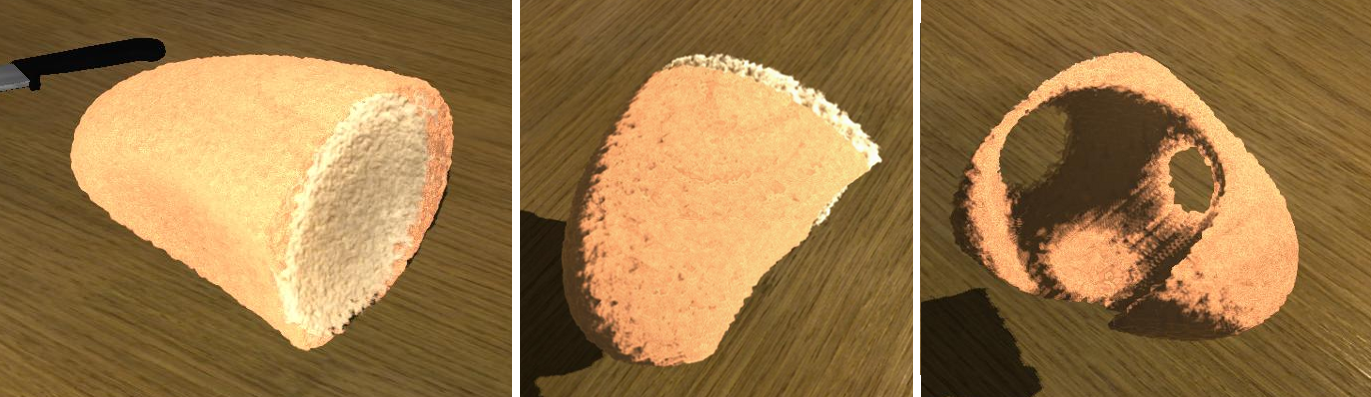
\includegraphics[width=13cm]{figures/crusts}}
%  \caption[Determinación de la corteza del pan utilizando morfología matemática]{Determinación de la corteza del pan utilizando morfología matemática. La imagen de la derecha muestra que el método se comporta adecuadamente incluso en casos donde existen grandes agujeros en la textura volumétrica.}
%  \label{fg:crusts}
%\end{figure}

\subsection{Tiempos de cómputo}
En la implementación utilizamos los lenguajes Python\footnote{python.org} y Cython\footnote{cython.org}.
En la Tabla~\ref{tab:computingtimes} se muestran tiempos de cómputo típicos para los distintos pasos en la simulación de la formación del pan, detallados en secciones anteriores. %In addition, rendering times with DVR are in the order of $~300$ ms (milliseconds), achieving interactive framerates.

\begin{table}[h!]
       % Give a unique label
% For LaTeX tables use
\begin{tabular}{lllll}
\hline\noalign{\smallskip}
Resolución de la Textura Volumétrica & $256^{3}$ & $384^{3}$  & $512^{3}$ \\
\noalign{\smallskip}\hline\noalign{\smallskip}
Leudado & 3.62 & 12.07 & 31.29 \\
Intersección & 8 & 10.27 & 14.97 \\
Transformación de Distancia & 7 & 23.73 & 56 \\
Cocción  & 49.81 & 144.69 & 313.7 \\
\hline\noalign{\smallskip}
Total & 68.43 & 190.76 & 415.96 \\
%Rendering & 1s & 4s & 0\% \\
\noalign{\smallskip}\hline
\end{tabular}
\caption{Tiempos de cómputo típicos en de las distintas etapas de la fabricación sintética de pan, expresados en segundos.}
\label{tab:computingtimes}
\end{table}

Es importante mencionar que la mayor parte del tiempo de cómputo en la cocción está dedicado al cómputo del gradiente, y no al proceso de cocción en sí.
Debido a los costos computacionales en resoluciones superiores, el usuario puede generar vistas previas de los panes utilizando campos escalares con menores resoluciones.


\subsection{Resultados}

En esta sección presentamos imágenes de geometrías de pan obtenidas utilizando nuestro modelo, renderizadas con el método presentado en el siguiente capítulo.
Los colores de corteza y miga son parámetros definibles por el usuario. Los cortes en la miga son fácilmente producidos anulando las regiones deseadas en la textura volumétrica luego de la cocción, y antes del renderizado.

Las Figs.~\ref{fg:renders}{-{}-}\ref{fg:bakingdeform2} muestran imágenes de los volúmenes obtenidos por medio del proceso de formación presentado, renderizados utilizando DVR.
Las Figs.~\ref{fg:renders} y ~\ref{fg:renders2} marcan las diferencias en calidad de la imagen resultante entre una versión de baja resolución ($256^{3}$) y una de alta resolución ($512^{3}$) respectivamente.
La Fig.~\ref{fg:renders3} muestra versiones de alta resolución de otras geometrías de panes.
La Fig.~\ref{fg:bakingcolors} muestra la misma corteza con diferentes historias de cocción.
Este efecto se logra definiendo diferentes valores máximos en el canal $L$ del espacio de color $CIELab$ para cada imagen.
Las Figs.~\ref{fg:bakingdeform} y \ref{fg:bakingdeform2} muestran el efecto de definir distintos valores del parámetro $S$ en la ec.~(\ref{Eq:rise}), los cuales producen distintos crecimientos de la masa.
Las imágenes muestran que el método produce imágenes realistas incluso para masas inverosímiles como una con forma de conejo.
El método permite realizar fácilmente cortes y tajadas en el modelo, definiendo como $0$ diferentes regiones en el volumen luego de la cocción y antes del renderizado.

Respecto de la sección anterior, puede observarse una forma más suave en las burbujas resultantes, junto con la capacidad de modelar tipos arbitrarios de panes.
Además, el proceso está basado en la secuencia real de pasos de la fabricación del pan, permitiendo la obtención de imágenes en distintos momentos del mismo.

\begin{figure*}[!ht]
\begin{center}
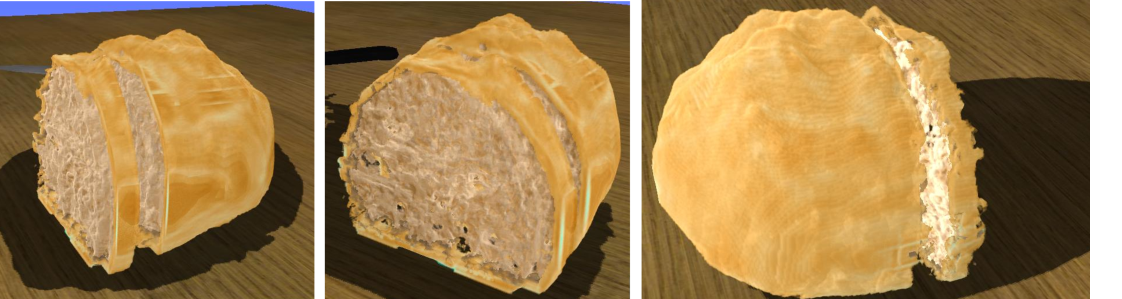
\includegraphics[width=13cm]{figures/Fig10}
\caption{Panes cortados luego de la cocción, utilizando una textura volumétrica de dimensiones $256^{3}$.}
\label{fg:renders}
\end{center}
\end{figure*}

\begin{figure*}[!ht]
\begin{center}
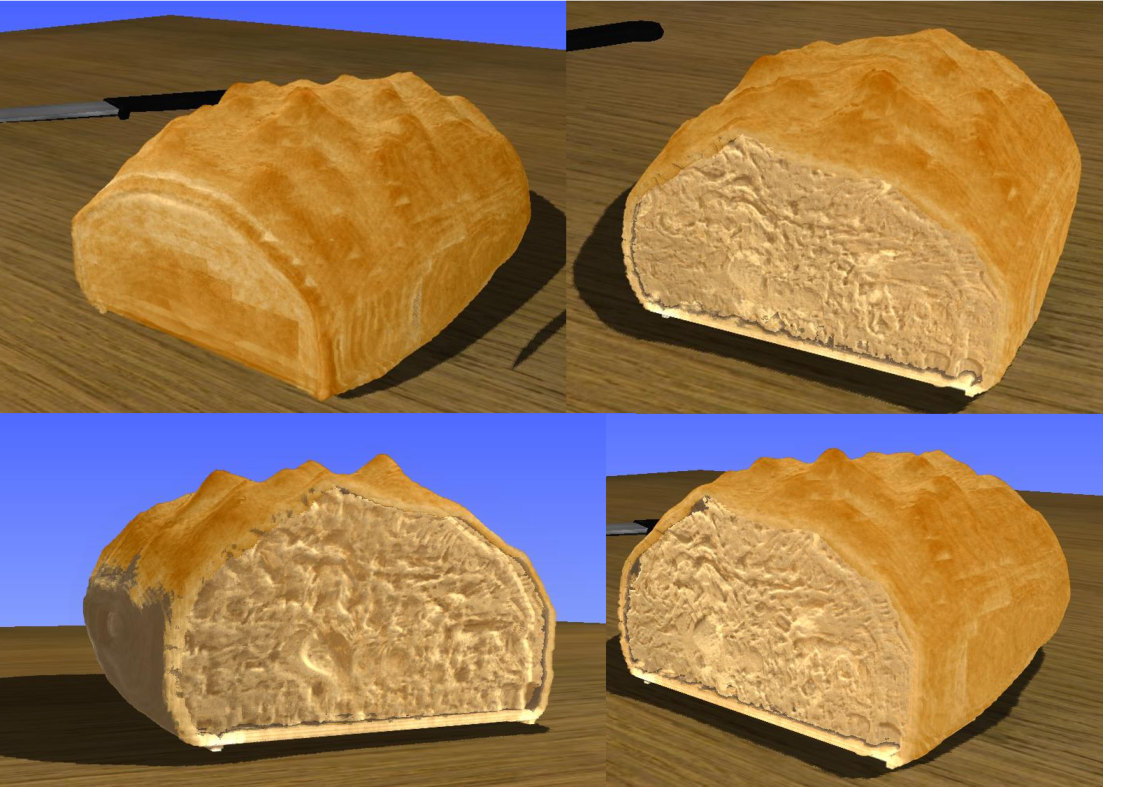
\includegraphics[width=13cm]{figures/Fig11}
\caption[Panes cortados luego de la cocción, utilizando una textura volumétrica de dimensiones $512^{3}$]{Panes cortados luego de la cocción, utilizando una textura volumétrica de dimensiones $512^{3}$. La miga muestra mayor detalle. Además el parámetro $S$ fue elegido con un valor aleatorio en cada punto, produciendo picos visibles en la corteza. El color de la corteza difiere ligeramente del de la figura anterior.}
\label{fg:renders2}
\end{center}
\end{figure*}

\begin{figure*}[!ht]
\begin{center}
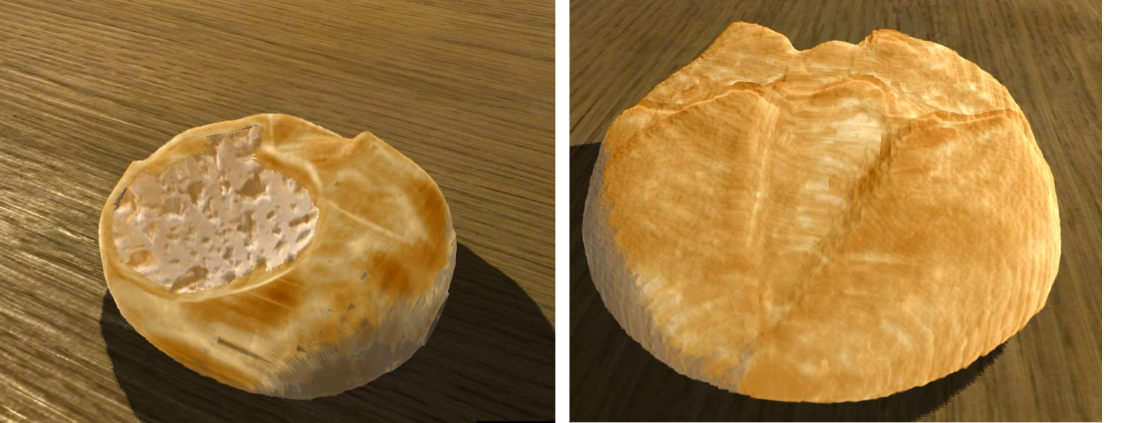
\includegraphics[width=13cm]{figures/Fig12}
\caption[Panes luego de la cocción]{Panes luego de la cocción. Se observan distintas geometrías $\rm 3D$ y apariencias de corteza.}
\label{fg:renders3}
\end{center}
\end{figure*}

\begin{figure*}[!ht]
\begin{center}
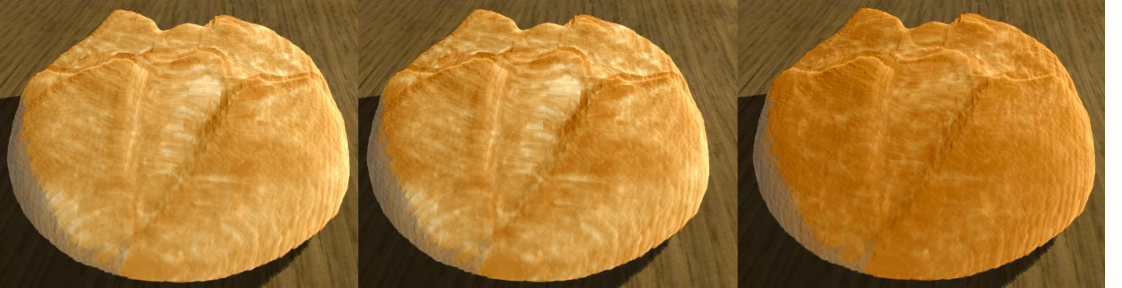
\includegraphics[width=13cm]{figures/Fig13}
\caption[Corteza con diferentes historias de cocción]{Cortezas con diferentes historias de cocción. De izquierda a derecha, se decrementa el valor máximo admitido para el canal $L$.}
\label{fg:bakingcolors}
\end{center}
\end{figure*}


\begin{figure*}[!ht]
\begin{center}
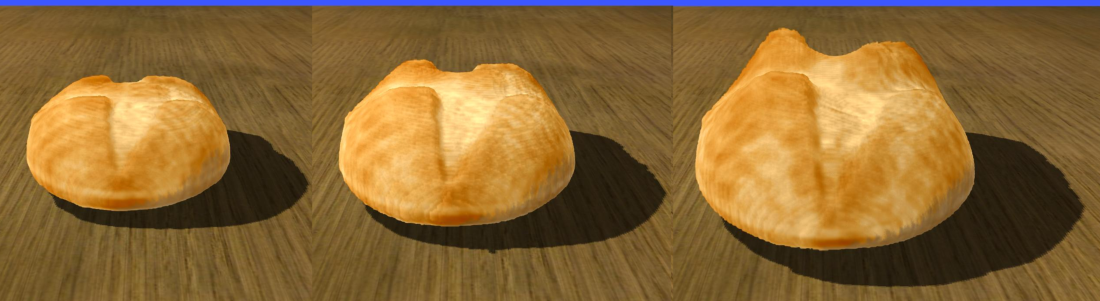
\includegraphics[width=13cm]{figures/Fig14}
\caption[Panes luego de la cocción mostrando diferentes crecimientos]{Panes luego de la cocción mostrando diferentes crecimientos. De izquierda a derecha se incrementa el parámetro $S$.}
\label{fg:bakingdeform}
\end{center}
\end{figure*}

\begin{figure*}[!ht]
\begin{center}
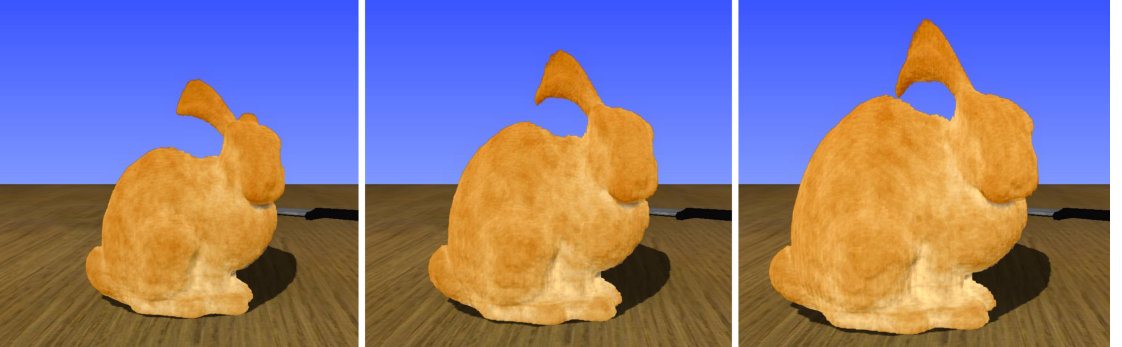
\includegraphics[width=13cm]{figures/Fig15}
\caption[Panes con forma de conejo luego de la cocción, mostrando diferentes crecimientos]{Panes con forma de conejo luego de la cocción, mostrando diferentes crecimientos. De izquierda a derecha se incrementa el parámetro $S$. Las imágenes resultan realistas incluso para masas de formas inverosímiles.}
\label{fg:bakingdeform2}
\end{center}
\end{figure*}


\section{Conclusiones}
En este Cap\'itulo hemos introducido diversos algoritmos para subsanar la falta de procedimientos flexibles e intuitivos para modelar determinados materiales, entre ellos materiales porosos como el pan. Además, como sub-producto de la investigación, se obtuvieron representaciones bidimensionales de madera, granito, mármol y otros materiales comunes en la literatura.
Hemos demostrado visualmente la capacidad de los métodos.

El primer aporte constituye un algoritmo que produce texturas bidimensionales de materiales conocidos como madera y granito, utilizando sistemas de partículas, el cual fue presentado en una conferencia local \cite{Baravalle2011}.
Haciendo hincapié en materiales porosos, particularmente el pan, diseñamos algoritmos que utilizan sistemas de partículas en conjunción con Sistemas Dinámicos para producir texturas que representan de manera realista geometrías de pan, el cual fue presentado en un congreso y revista nacionales \cite{Baravalle2014}.

Finalmente, utilizando como referencia el proceso de formación real del pan, utilizamos conocimientos de ingeniería de los alimentos para producir una secuencia de pasos que emulan el proceso real de formación del pan, el cual fue presentado en una revista internacional \cite{Baravalle2015_2}.
El mismo permite modelar de manera realista tipos de panes arbitrarios, produciendo geometrías de su miga y su corteza, utilizando un proceso fractal de generación.
Para ello, emulamos un proceso de leudado configurable por el usuario, tanto en forma global, supliendo una geometría arbitraria en tres dimensiones, como en el burbujeado interno, por medio de parámetros intuitivos de generación (radio máximo y mínimo de las burbujas, cantidad de burbujas, etc.).
Luego aplicamos una simulación física de la cocción, la cual se utilizó para deformar ligeramente las burbujas, siguiendo las líneas definidas por la forma exterior del pan, y producir una simulación del levantamiento del mismo, debido a las burbujas atrapadas en su volumen.
Finalmente, la corteza fue generada sobre la superficie del material.
El algoritmo de renderizado utilizado será explicado en el siguiente capítulo, el mismo produjo imágenes realistas de diversos tipos de pan, en varias etapas del proceso de formación del mismo.

El modelo introducido resulta más flexible y poderoso que aquéllos del estado del arte actual en modelado de geometría de materiales porosos y panes.
En un capítulo posterior, y con intención de validar el procedimiento, mostraremos que las geometrías obtenidas por el método inspirado en el proceso de formación del pan, arrojan distribuciones de burbujas coincidentes con panes reales.

